Sensitivity analysis identifies how and the extent to which variations 
in model input parameters affect select performance 
metrics of the fuel cycle. Additionally, it reveals the combined effect 
of varying multiple parameters on 
an output metric. This information can then be used to design 
an optimized transition scenario by identifying which input parameters 
will affect the results the most, and how these parameters should be 
changed to obtain desired results (e.g., minimizing \gls{HALEU} requirements
of a transition). 

\section{Methodology}
We performed sensitivity analysis on Scenario 7 (once-through fuel cycle 
transition to Xe-100, VOYGR, and \gls{MMR} with a no growth energy demand) 
using a coupling between \Cyclus with Dakota \cite{adams_dakota_2021}, an 
open-source code developed by \acrfull{SNL} for uncertainty quantification, 
sensitivity analysis, and optimization. This coupling mirrors  
the scripts in the \texttt{dcwrapper} GitHub repository 
\cite{chee_arfcdcwrapper_2019}. We performed three different types 
of sensitivity analysis: \acrfull{OAT}, synergistic, 
and global. \gls{OAT} analysis varies a single input parameter to 
investigate the effect of each parameter individually. In the context of 
this work, synergistic 
analysis varies two input parameters at once to investigate how the 
interaction of the two parameters affects the results. Finally, the global 
sensitivity
analysis varies more than two input parameters to provide a holistic 
view of how multiple parameters interact and affect the output metrics. 
For this work, we considered variations in the transition 
start time, the build share of each type of advanced reactor, 
the \gls{LWR} lifetimes, and the discharge burnup of fuel from the 
\gls{HALEU}-fueled reactors. 

The transition start time ranges from January 
2025 to January 2040 in three-month intervals, but the same energy demand 
is specified for all perturbations (87.20 GWe-yr). We consider this parameter 
to provide a relaxation of the aggressive 2025 transition start date 
used in the transition analysis of Chapters \ref{ch:once_through_results} and
\ref{ch:recycle_results}.

We consider three 
iterations of the build share, once for each advanced reactor, with 
build share percentages ranging from 0-50\% 
in increments of 5\%. To account for the build share of an advanced reactor,
we adjusted the deployment scheme described in Section \ref{sec:once-through-methods}.
Instead of the reactor type with the largest power output 
deployed first, the reactor with the specified build share is deployed first 
until the build share is met. Then the remaining two advanced reactor types are 
deployed in the manner described in Section \ref{sec:once-through-methods},
with the larger of the two remaining reactors preferentially deployed and 
the smaller reactor deployed last to meet or exceed the power demand. Figure 
\ref{fig:build-share-deploy} illustrates how we applied this deployment 
scheme to meet a fictional demand of 530 MWe and a VOYGR build share of 
50\%. We vary this parameter of the transition because of the large effect 
of the advanced reactors deployed in each of the transition scenarios. 
Unless an advanced reactor build share is specified, this analysis 
applies the same advanced reactor deployment schedule as Scenario 7
(see Section \ref{sec:nogrowth_reactors}).

\begin{figure}
    \centering 
    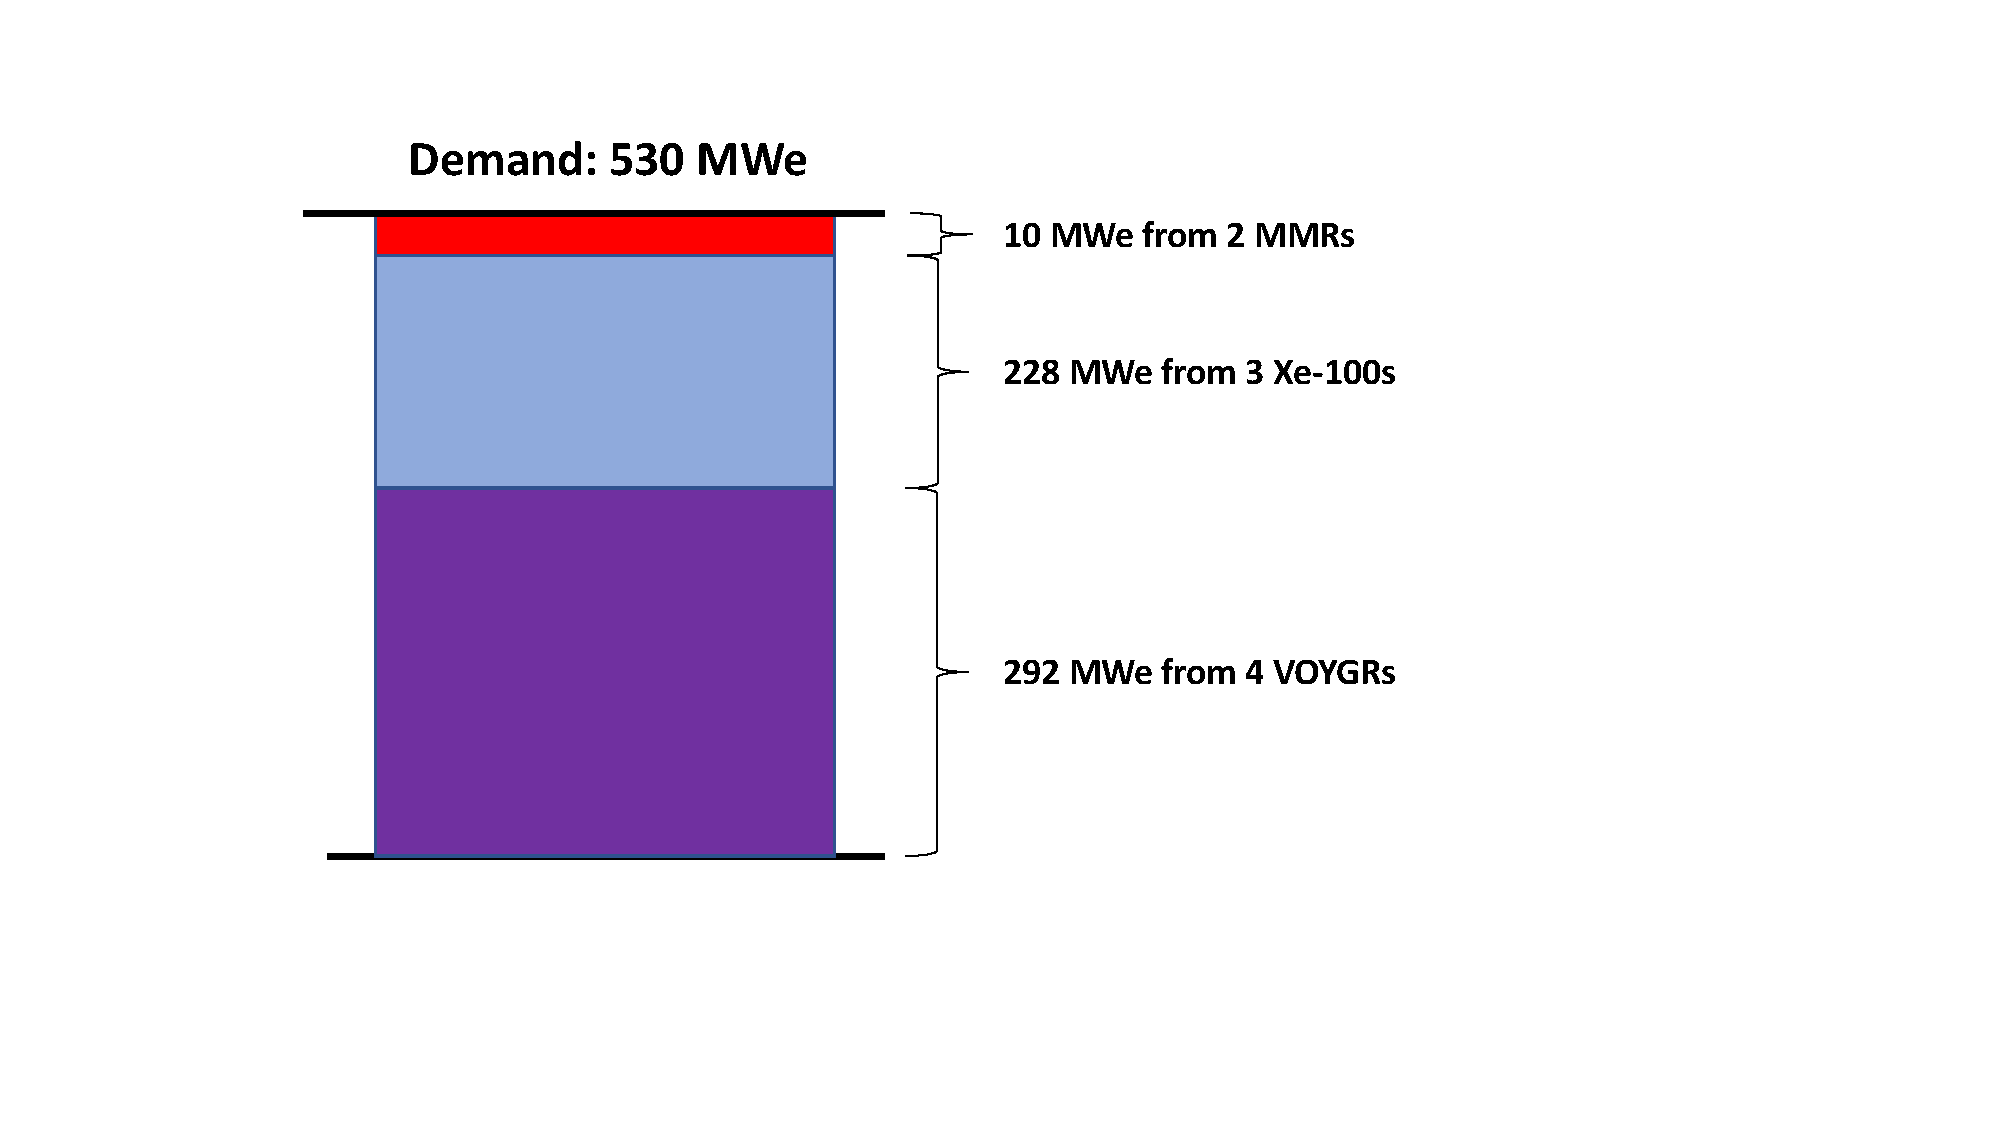
\includegraphics[scale=0.5, trim=50 100 100 0,clip]{VOYGR_build_share.pdf}
    \caption{Demonstration of the adjusted advanced reactor deployment 
    scheme to meet a demand of 530 MWe and a VOYGR build share of 
    50\%.}
    \label{fig:build-share-deploy}
\end{figure}

The \gls{LWR} lifetimes are varied based 
on the percent of the fleet that operate for 80 years. This 
variable varies between 0-50\%, in increments of 5\%, of the \gls{LWR} 
fleet operating for 80 
years, while the other \glspl{LWR} operate for 60 years. This input 
parameter reflects the effects of different numbers of \glspl{LWR} 
receiving license extensions to 80 years. Various utilities are exploring 
and pursuing license extensions for \glspl{LWR}, so including this parameter 
reflects this occurrence. The 
\glspl{LWR} do not all start operation at the same time, so the 
selection of the \glspl{LWR} that operate for 80 years affects the results, 
even if the number is the same. Therefore, reactors are prioritized based 
on their power outputs for the lifetime extensions, reflecting the greater likelihood of 
larger units receiving a license extension. Previous sensitivity analysis of 
fuel cycle transitions considered the impact of the transition start time 
and the \gls{LWR} lifetimes \cite{chee_sensitivity_2019,feng_sensitivity_2020},
which provides some basis for why these input parameters were selected for this 
work.

Finally, we varied the discharge burnup of the two \gls{HALEU}-fueled 
reactors in this work (the Xe-100 and \gls{MMR}) because these two reactors 
are reaching burnup levels larger than the \gls{NRC}-approved 62 MWd/kgHM 
\cite{noauthor_higher_2023}. Therefore, it is possible that these 
reactors would need to be operated under different conditions until
higher burnups are approved by the \gls{NRC}.
Therefore, inclusion of this variable explores the impact 
on resource needs if these reactors are prohibited from achieving 
their 
reported burnup values. This analysis is not performed for the VOYGR because this 
design aims to achieve a burnup that is within the \gls{NRC} limit. 

To vary the burnup of the Xe-100, we considered two difference approaches. The 
first approach was to vary the number of passes through the core for each pebble 
while keeping the length of each pass and the total mass of uranium 
in the core constant (i.e., reducing the number of batches). Varying the 
number of passes between one and six 
results in discharge burnup values of 28, 56, 84, 112, 140, and 168 MWd/kgU, 
using Eq. \ref{eq:fuel_mass}. This approach provides a coarse grid 
for the burnup values that reflects possible changes to meet current 
\gls{NRC} regulations. The second approach varies the length 
of each pass by one month, while keeping the number of passes and the 
total mass of uranium 
constant. This approach provides a more fine grid around the declared 
burnup value, reflecting potential small variations in reactor operation. 
The second approach results in burnup values of 151 and 185 MWd/kgU, 
which are about $\pm$10\% of the stated discharge burnup of 168 MWd/kgU. 

To vary the \gls{MMR} burnup, we varied the cycle time (and thus lifetime) of 
the reactor while the total mass of uranium was held constant. 
Cycle times of 10, 15, and 20 years were considered, resulting in burnup 
values of 41, 62, and 82 MWd/kgU. Additionally, the lifetime was varied to 
result in burnup values $\pm$10\% and $\pm$5\% around the stated burnup of 
82 MWd/kg, resulting in burnup values of 74, 78, 86, and 90 MWd/kgU. 

The sensitivity analysis focuses on the effects of these input parameters 
on the following metrics: the amount of waste generated that 
must be sent to a repository (\gls{UNF} mass), the mass of enriched uranium, 
the mass of \gls{HALEU},
the amount of \gls{SWU} capacity required to produce all enriched uranium, the 
\gls{SWU} capacity required to produce \gls{HALEU}, and the feed uranium 
required to produce \gls{HALEU}. We considered each of these metrics 
within the transition analysis, allowing for comparison between Chapters 
\ref{ch:once_through_results}, \ref{ch:recycle_results}, and this chapter. 
We compare each metric based on the cumulative sum required, starting 
at the transition start time. 

\section{One-at-a-time}\label{sec:ot_oat}
This section discusses the results of the \gls{OAT} sensitivity analysis 
as applied to Scenario 7. A subset of this analysis is presented 
in \cite{bachmann_sensitivity_2022}, but the analysis presented here has 
an expanded scope and updated methodology to address the non-consistent 
replacement of advanced reactors in the previously published work.
The results in this subsection focus on 
the relative change in each metric for each parameter varied, because 
of the large range of the metric values. To that end, Table 
\ref{tab:oat_values} reports the minimum, 
average, and maximum value for each metric.

\begin{table}[ht!]
    \centering
    \caption{Minimum, average, and maximum value of each metric caused 
    by the variation of each parameter.}
    \label{tab:oat_values}
    \begin{tabular}{llrrrl}       
        \hline 
        Parameter &     Metric &      Minimum &      Average &      Maximum & Units\\
        \hline
        Transition Start &  Fuel Mass & 2.832e+07 & 3.001e+07 & 3.086e+07 & kg \\
                         & HALEU Mass & 2.777e+07 & 2.931e+07 & 3.005e+07 & kg\\ 
                         &  Total SWU & 9.727e+08 & 1.036e+09 & 1.068e+09 & kg-SWU\\ 
                         & HALEU SWU & 9.690e+08 & 1.031e+09 & 1.062e+09 & kg-SWU\\
                         &        UNF & 2.600e+07 & 2.744e+07 & 2.813e+07 & kg\\  
                         & HALEU Feed & 8.406e+08 & 8.936e+08 & 9.204e+08 & kg\\\hline
        LWR Lifetimes &  Fuel Mass & 2.226e+07 & 2.574e+07 & 2.934e+07 & kg\\
                      & HALEU Mass & 2.186e+07 & 2.528e+07 & 2.885e+07 & kg\\
                      &  Total SWU & 7.780e+08 & 8.973e+08 & 1.021e+09 & kg-SWU\\
                      &  HALEU SWU & 7.753e+08 & 8.941e+08 & 1.018e+09 & kg-SWU\\
                      &        UNF & 1.956e+07 & 2.305e+07 & 2.669e+07 & kg\\
                      & HALEU Feed & 6.716e+08 & 7.746e+08 & 8.820e+08 & kg\\\hline 
        Xe-100 Build Share &  Fuel Mass & 8.230e+07 & 1.130e+08 & 1.471e+08 & kg\\
                           & HALEU Mass & 2.827e+06 & 1.078e+07 & 1.804e+07 & kg\\
                           &  Total SWU & 1.083e+09 & 1.090e+09 & 1.102e+09 & kg-SWU\\
                           &  HALEU SWU & 1.275e+08 & 3.999e+08 & 6.501e+08 & kg-SWU\\
                           &        UNF & 7.511e+07 & 1.032e+08 & 1.344e+08 & kg\\
                           & HALEU Feed & 1.081e+08 & 3.448e+08 & 5.622e+08 & kg\\\hline 
        MMR Build Share &  Fuel Mass & 3.702e+07 & 4.918e+07 & 6.134e+07 & kg\\
                        & HALEU Mass & 2.670e+07 & 3.852e+07 & 5.039e+07 & kg\\
                        &  Total SWU & 9.901e+08 & 1.600e+09 & 2.212e+09 & kg-SWU\\
                        &  HALEU SWU & 9.205e+08 & 1.528e+09 & 2.138e+09 & kg-SWU\\
                        &        UNF & 3.440e+07 & 4.066e+07 & 4.689e+07 & kg\\
                        & HALEU Feed & 7.995e+08 & 1.310e+09 & 1.822e+09 & kg\\\hline 
        VOYGR Build Share &  Fuel Mass & 3.045e+07 & 6.436e+07 & 9.510e+07 & kg\\
                          & HALEU Mass & 1.516e+07 & 2.233e+07 & 3.045e+07 & kg\\
                          &  Total SWU & 1.077e+09 & 1.082e+09 & 1.092e+09 & kg-SWU\\
                          &  HALEU SWU & 5.528e+08 & 7.988e+08 & 1.080e+09 & kg-SWU\\
                          &        UNF & 2.765e+07 & 5.870e+07 & 8.679e+07 & kg\\
                          & HALEU Feed & 4.775e+08 & 6.913e+08 & 9.353e+08 & kg\\\hline 
        Xe-100 Burnup &  Fuel Mass & 2.761e+07 & 5.888e+07 & 1.591e+08 & kg\\
                      & HALEU Mass & 2.681e+07 & 5.809e+07 & 1.583e+08 & kg\\
                      &  Total SWU & 9.559e+08 & 2.034e+09 & 5.489e+09 & kg-SWU\\
                      &  HALEU SWU & 9.505e+08 & 2.029e+09 & 5.484e+09 & kg-SWU\\
                      &        UNF & 2.486e+07 & 5.614e+07 & 1.564e+08 & kg\\
                      & HALEU Feed & 8.233e+08 & 1.760e+09 & 4.761e+09 & kg\\\hline 
        MMR Burnup &  Fuel Mass & 3.065e+07 & 3.124e+07 & 3.293e+07 & kg\\
                   & HALEU Mass & 2.986e+07 & 3.045e+07 & 3.214e+07 & kg\\
                   &  Total SWU & 1.059e+09 & 1.085e+09 & 1.162e+09 & kg-SWU\\
                   &  HALEU SWU & 1.054e+09 & 1.080e+09 & 1.156e+09 & kg-SWU\\
                   &        UNF & 2.791e+07 & 2.850e+07 & 3.019e+07 & kg\\
                   & HALEU Feed & 9.128e+08 & 9.354e+08 & 1.000e+9 & kg\\
        \hline
    \end{tabular}
\end{table}


\subsection{Transition start time}
Delays in the transition start time generally decrease all of the output 
metrics, as shown in Figure \ref{fig:ts_scenario7}. This result matches 
expectations, because if the advanced reactors are deployed for less time, 
then they require fewer resources. However, there are some oscillations in 
the output metrics between individual time steps. For example, a transition 
start time of October 2029 increases the fuel mass and \gls{UNF} mass 
relative to July 2029, the start time previous. This increase results 
from changes in the number 
of each advanced reactor deployed, because of differences in the gap 
between energy produced and energy demand that must initially be filled when 
advanced reactors are deployed. By waiting until October 2029, more VOYGRs 
are deployed than when the transition starts in July 2029. As discussed in 
Chapter \ref{ch:once_through_results}, the VOYGR needs a larger fuel mass, 
and thus discharges more \gls{UNF} than the Xe-100 and \gls{MMR}. Therefore, 
these two metrics increase for this particular transition start time. 

\begin{figure}[h!]
    \centering
    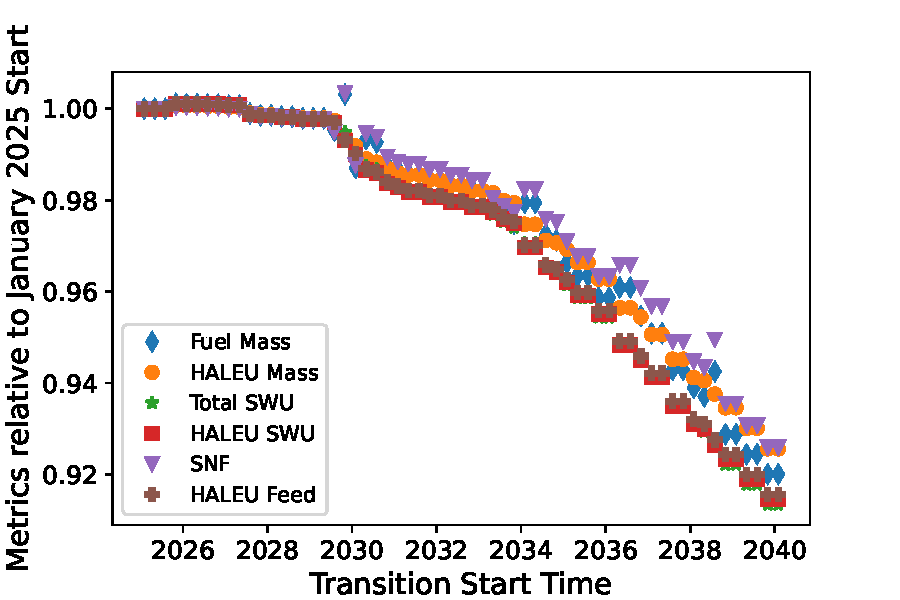
\includegraphics[scale=0.8]{ts.pdf}
    \caption{Change in each metric as a function of transition start 
    time, relative to a transition start in January 2025.}
    \label{fig:ts_scenario7}
\end{figure}

One of the disadvantages in delaying the transition start time is the 
increasing gap between energy supplied and energy demand as the transition 
start time is delayed. All of these scenarios have a constant demand 
of 87.20 GWe-yr beginning in January 2025. By delaying the transition start 
time to after September 2025 (the observed initial deployment time of advanced 
reactors in Section \ref{sec:nogrowth_reactors}), there is a difference
between the energy supplied and the energy demand. The largest gap observed 
is 36.7
GWe-yr, when reactors are deployed starting in January 2040. Therefore, 
delaying the transition start time is not an ideal method of 
potentially reducing materials to support advanced reactors. 

\subsection{LWR lifetimes}
The next metric varied is the percent of the \glspl{LWR} that operate for 
80 years, reflecting the effect license extensions in the \gls{LWR} fleet. 
Figure \ref{fig:lwr_scenario7} shows that the percent of the \gls{LWR} 
fleet operating for 80 years increases, all of the metrics decrease. 
All of the metrics decrease 
linearly and by a similar magnitude, with some variation because 
of changes in the number of each advanced reactor deployed, as discussed 
in Chapter \ref{ch:once_through_results}. The \gls{UNF} mass decreases 
more than the other metrics across 
this parameter space, ranging between 19.5-26.7 MTU.

\begin{figure}[h!]
    \centering
    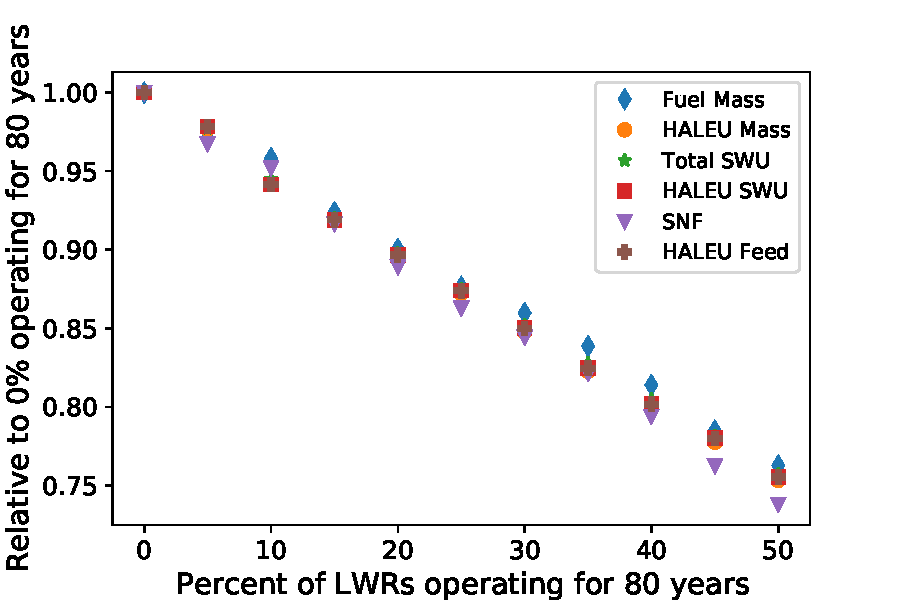
\includegraphics[scale=0.8]{lwr.pdf}
    \caption{Change in each metric as a function of percent of LWR fleet  
    operating for 80 years, relative to 0\%.}
    \label{fig:lwr_scenario7}
\end{figure}

Across this parameter space, the metrics decrease by a greater fraction than 
when varying the transition start time. The increased impact on the metrics 
is partly because of a small modeling change. When varying the transition 
start time, the \glspl{LWR} are assumed to have the same lifetime as the 
ones used in the transition analysis. Almost all of these lifetimes are  
60 years but there are a select few (such as Watts Bar Unit 2) that 
are currently licensed for 40 years. A simplifying assumption for 
modeling the effects of extending the \gls{LWR} lifetimes is that 
they operate for either 60 or 80 years, giving those select few reactors 
an artificial lifetime extension from 40 to 60 years, compared with the previous analysis. 
This modeling difference does not have a large impact on the results as 
evidenced by the maximum \gls{HALEU} mass when varying the \gls{LWR} lifetimes 
being only 4.9\% lower than the maximum \gls{HALEU} mass when varying the 
transition start time. Therefore, we can attribute most of the change in
the metrics to the 
change in the \gls{LWR} lifetimes and not the artificial increase in 
lifetimes from 40 to 60 years. Additionally, extending the \gls{LWR}
lifetimes inherently delays the start time of the transition, or at 
least decreases the speed of the transition, because the \glspl{LWR} 
are sufficient to meet the energy demand for a longer period of time.
In addition to causing greater change in the metrics, the energy demand 
is always met when varying the \gls{LWR} lifetimes, which suggests that 
extending the lifetimes of the \glspl{LWR} is a preferable parameter to vary 
if one wishes to decrease material requirements of this transition. 

\subsection{Xe-100 build share}
Figure \ref{fig:xe100_scenario7} shows that as the Xe-100 build share increases, 
the \gls{HALEU}-related metrics 
increase while the total \gls{UNF} and total fuel mass decrease and the 
total \gls{SWU} capacity stays relatively constant. Figure \ref{fig:xe100_s7_combined_reactors} 
shows that as the Xe-100 build share 
increases, the number of \glspl{MMR} is relatively constant and the number of 
VOYGRs decreases. These results show that as the Xe-100 build share 
increases, the Xe-100s are primarily replacing power that is supplied by 
the VOYGRs, instead of a portion of both of the other advanced reactors.
This replacement of VOYGRs is because of the deployment scheme used in this
work, as the VOYGR has the largest power output between the VOYGR and 
\gls{MMR}. Therefore, VOYGR deployment is maximized when the Xe-100 
build share is 0\%. This effect of the deployment scheme indicates that 
varying this parameter highlights trade-offs between the Xe-100 and 
VOYGR reactors.

\begin{figure}[h!]
    \centering
    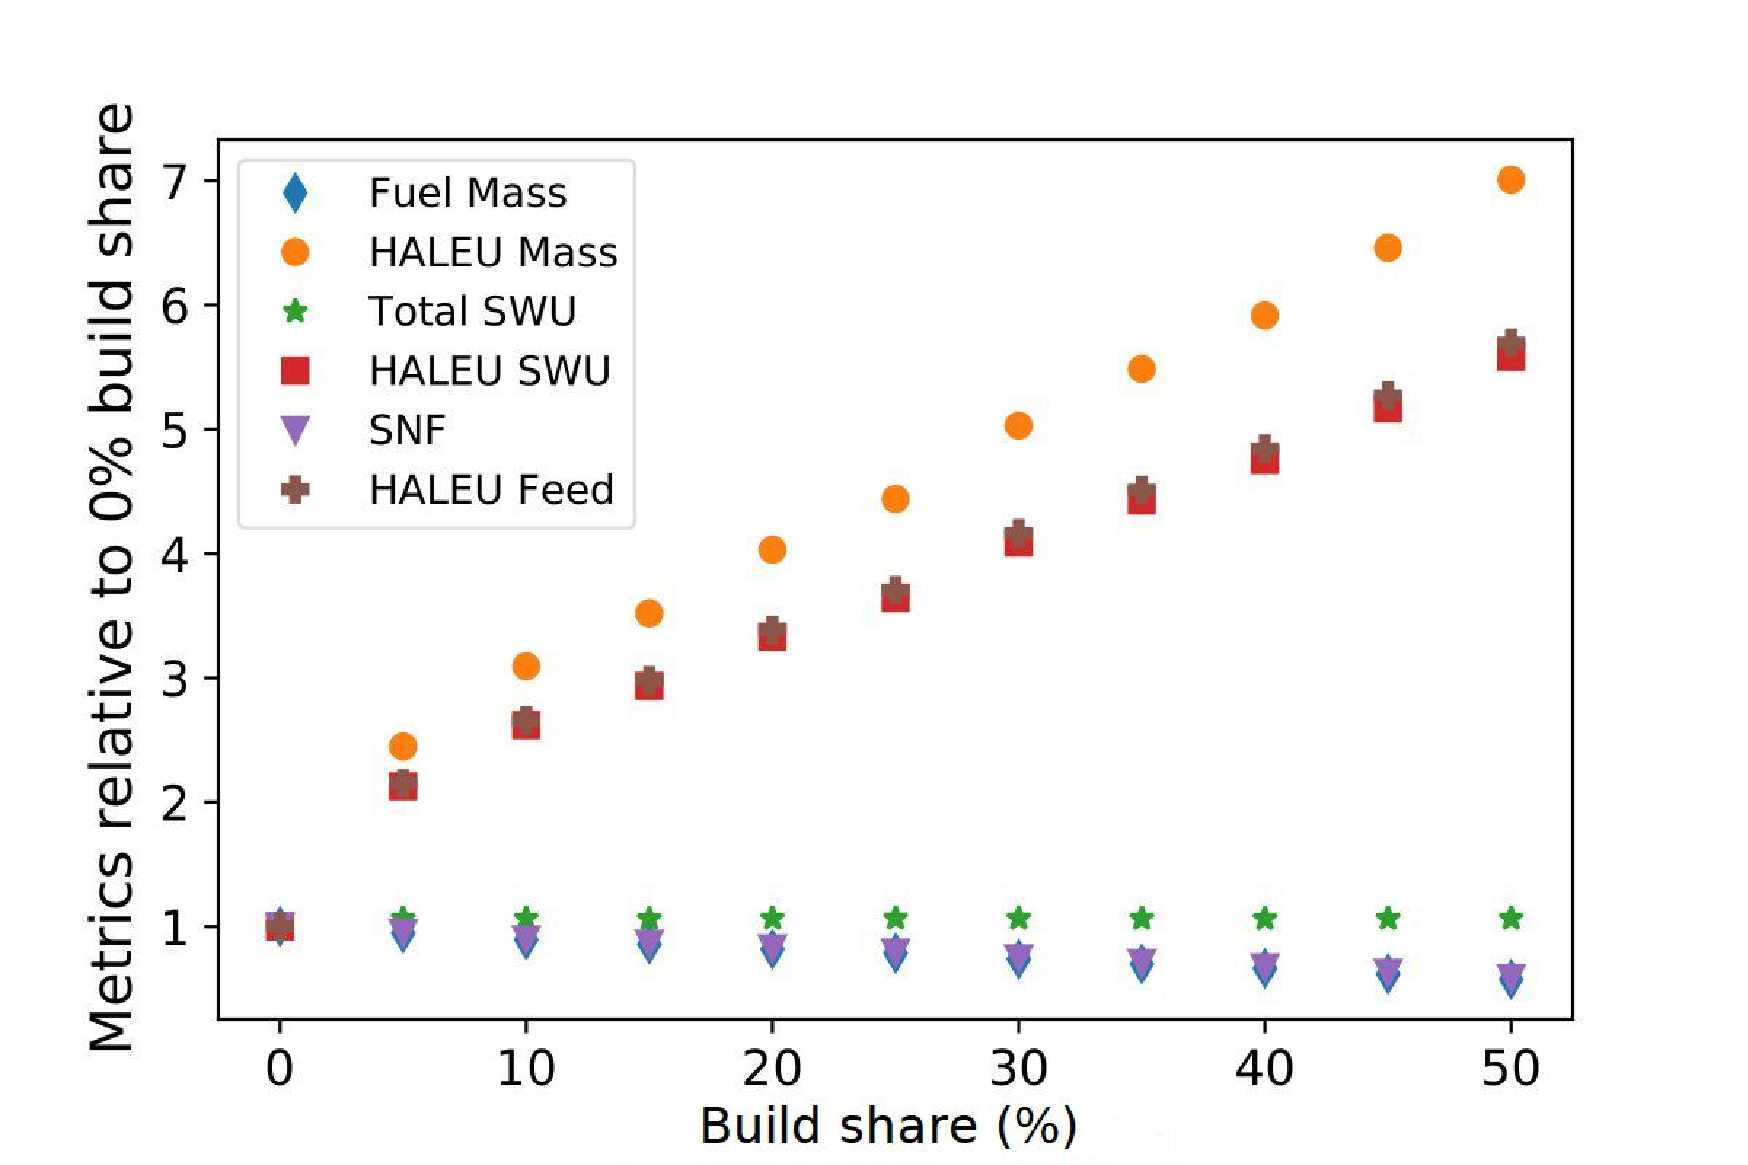
\includegraphics[scale=0.45]{xe100.pdf}
    \caption{Change in each metric as a function of Xe-100 build share, 
    relative to a build share of 0\%.}
    \label{fig:xe100_scenario7}
\end{figure}

\begin{figure}[h!]
    \centering
    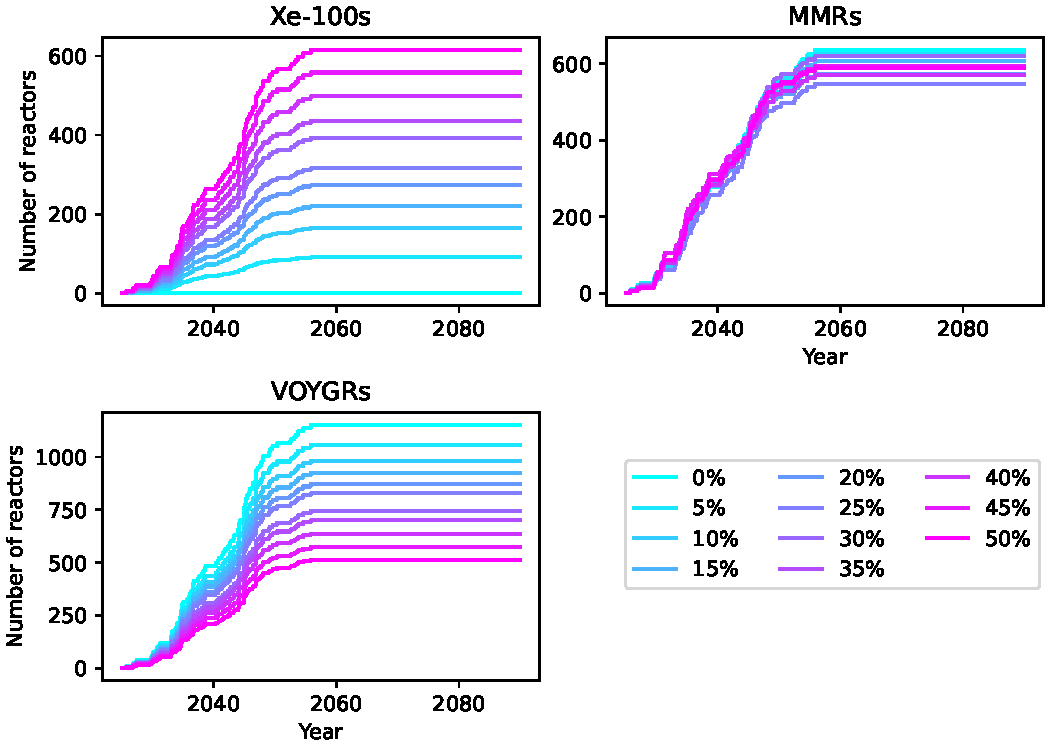
\includegraphics[scale=0.7]{xe100_combined_reactors.pdf}
    \caption{Number of Xe-100s (top left), MMRs (top right), and VOYGRs
    (bottom left) as a function of Xe-100 build share.}
    \label{fig:xe100_s7_combined_reactors}
\end{figure}

The \gls{HALEU}-related metrics increase with Xe-100 build share because more of 
the demand is met through advanced reactors requiring \gls{HALEU}. The total 
fuel mass and \gls{UNF} mass decrease because the 
Xe-100 requires less fuel per unit time and energy than the VOYGR, as discussed 
in Chapter \ref{ch:once_through_results}. The total \gls{SWU} capacity required 
is relatively constant, decreasing between 0.3-1.7\% compared to the \gls{SWU} capacity 
required for a 0\% Xe-100 build share. This stagnant behavior of the total 
\gls{SWU} capacity is consistent with the similar \gls{SWU} capacity required 
by Scenarios 3-7 in Section \ref{sec:nogrowth_swu}, when either the Xe-100 or 
VOYGR are primarily deployed. These results highlight the trade-off between the
\gls{HALEU}-related metrics and the total fuel mass and \gls{UNF} mass in deploying 
the Xe-100 versus the VOYGR. Both reactors require similar \gls{SWU} capacities 
but because of the different product assays required, the cascade configuration 
will vary. The \gls{HALEU}-related metrics increase up to 638\% of the 
mass required 
for a 0\% Xe-100 build share. The total fuel mass and \gls{UNF} mass decrease 
to up to 44.11\% of the mass required for 1 0\% Xe-100 build share. 

\subsection{MMR build share}
All of the metrics increase with increasing \gls{MMR} share, as shown 
in Figure \ref{fig:mmr_scenario7}. As the \gls{MMR} build share 
increases, the total \gls{SWU}, \gls{HALEU} \gls{SWU}, 
and \gls{HALEU} feed have the greatest relative increase because more of the 
advanced reactor fleet uses the highest enrichment level of the three 
advanced reactors. The \gls{HALEU} mass 
increases with the \gls{MMR} build share \glspl{MMR} replace Xe-100s
as the build share increases, shown in  
Figure \ref{fig:mmr_reactors_s7}.
The \gls{MMR} requires a greater fuel mass than the Xe-100, causing the increase 
in the \gls{HALEU} mass as \glspl{MMR} replace Xe-100s. 
The larger fuel mass required by the \gls{MMR}, compared 
with the Xe-100, compounds with the higher enrichment required by the \gls{MMR} 
to cause the greater relative increase in the total \gls{SWU}, \gls{HALEU} \gls{SWU}, 
and \gls{HALEU} feed. 

\begin{figure}[h!]
    \centering
    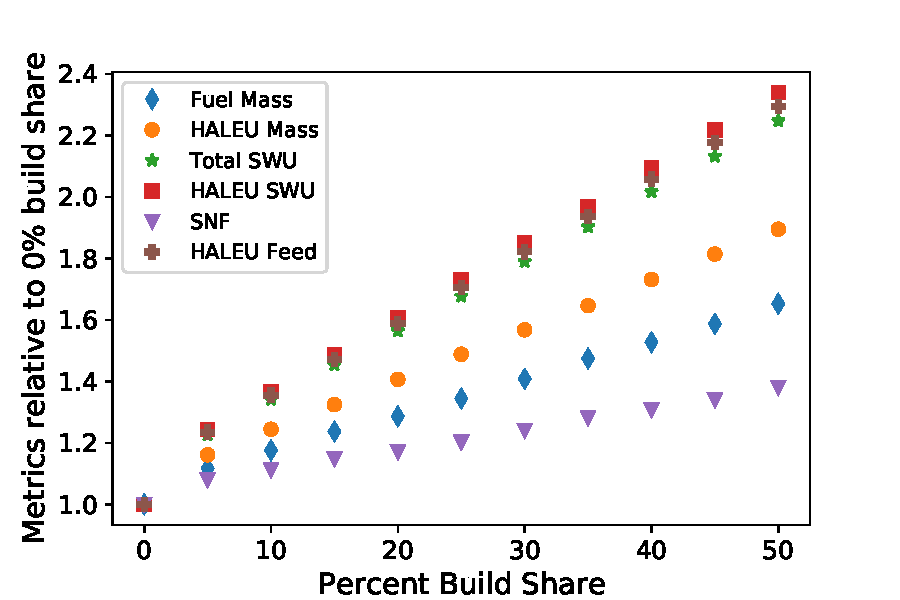
\includegraphics[scale=0.45]{mmr.pdf}
    \caption{Change in each metric as a function of MMR build share, 
    relative to a build share of 0\%.}
    \label{fig:mmr_scenario7}
\end{figure}


\begin{figure}[h!]
    \centering
    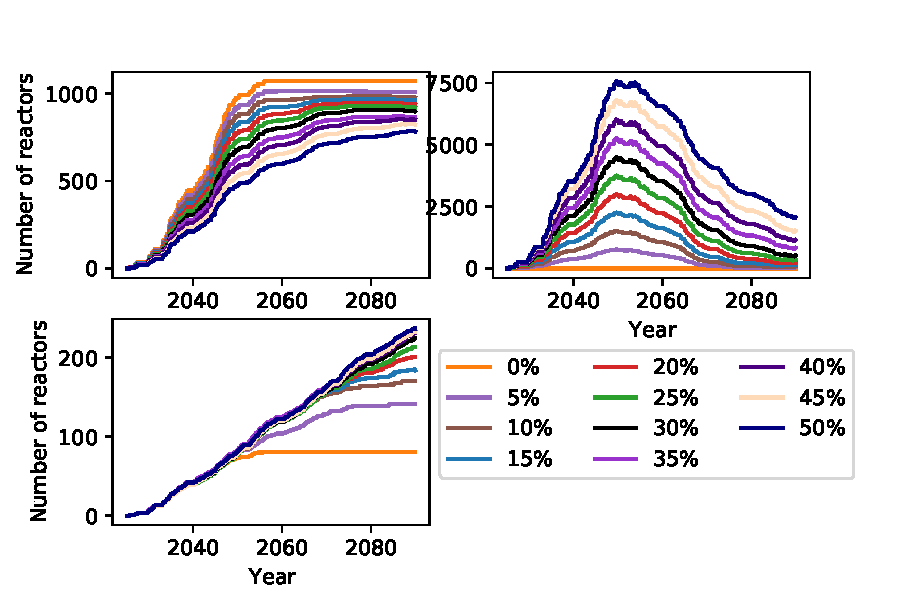
\includegraphics[scale=0.7]{mmr_combined_reactors.pdf}
    \caption{Number of Xe-100s (top left), MMRs (top right), and 
    VOYGRs (bottom left) deployed as a function of time and 
    MMR build share.}
    \label{fig:mmr_reactors_s7}
\end{figure}

The \gls{UNF} mass does not experience the same 
relative increase as the total fuel mass because any fuel that is still in a 
reactor core at the end of the simulation is not accounted for in the 
\gls{UNF} mass. Therefore, as the \gls{MMR} build share increases, more 
of the enriched uranium sent to reactors is still in a reactor core
at the end of the simulation because of the long cycle time of the 
\gls{MMR}. 
Based on the replacement of Xe-100s with \glspl{MMR} as the \gls{MMR} 
build share increases, these results highlight the effects of deploying the
\gls{MMR} over the Xe-100. 

\subsection{VOYGR build share}
Varying the VOYGR build share causes trends that are opposite 
to the effects observed from varying the Xe-100 build share. 
(Figure 
\ref{fig:voygr_scenario7}). The total fuel mass and \gls{UNF} mass 
increase, the \gls{HALEU}-related metrics decrease, and the total 
\gls{SWU} capacity remains relatively constant. This reversal 
of trends occurs because there is a replacement of Xe-100s with VOYGRs
with increasing build share (Figure \ref{fig:voygr_reactors_s7}), 
the opposite of what happens with an increasing Xe-100 build share. 

\begin{figure}[h!]
    \centering
    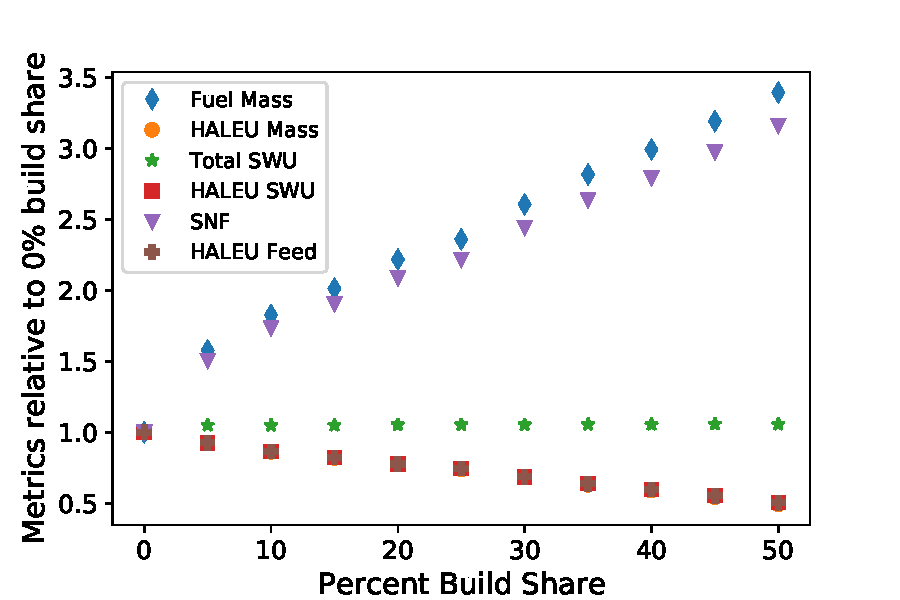
\includegraphics[scale=0.45]{voygr.pdf}
    \caption{Change in each metric as a function of VOYGR build share, 
    relative to a build share of 0\%.}
    \label{fig:voygr_scenario7}
\end{figure}

\begin{figure}[h!]
    \centering
    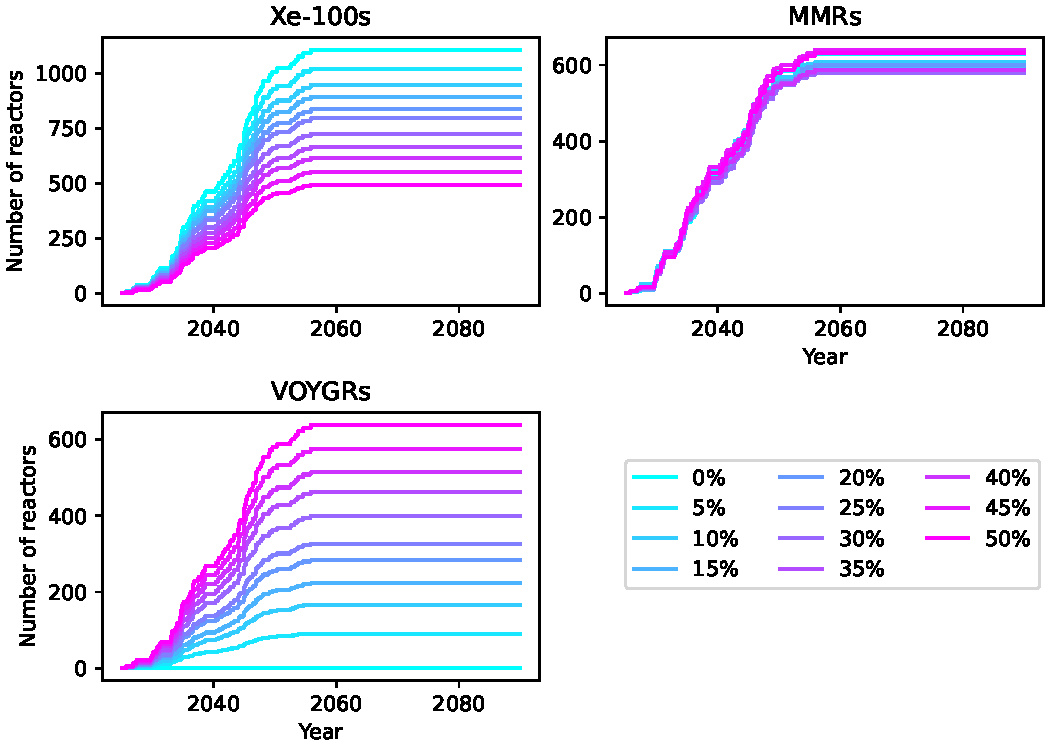
\includegraphics[scale=0.7]{voygr_combined_reactors.pdf}
    \caption{Number of Xe-100s (top left), MMRs (top right), and 
    VOYGRs (bottom left) deployed as a function of time and 
    VOYGR build share.}
    \label{fig:voygr_reactors_s7}
\end{figure}

The total \gls{SWU} capacity required varies between 99.6\%-101.2\% of the 
\gls{SWU} capacity needed for a 0\% VOYGR build share, a range of 1.077$\times 10^9$
- 1.092$\times 10^9$ kg-SWU (Table \ref{tab:oat_values}). The total fuel mass 
and \gls{UNF} mass increase 
up to 313.9\% of the mass required for a 0\% VOYGR build share, and the 
\gls{HALEU}-related metrics decrease to 49.77\% of the mass required 
for a 0\% VOYGR build share. The \gls{UNF} and total fuel masses increase 
because the VOYGR requires more fuel than the Xe-100, largely stemming from 
the difference in discharge burnup of these two reactors. The \gls{HALEU}-related 
metrics all decrease because the VOYGR does not require \gls{HALEU}. As the 
VOYGR build share increases a smaller portion of the advanced reactor fleet 
requires \gls{HALEU}. While the trends from varying the VOYGR build share 
mirrors the trends from varying the Xe-100 build share, the magnitude of the 
changes are not the same because these 
parameter variations cover adjacent but not overlapping design spaces. 

\subsection{Xe-100 burnup}
When varying the burnup of fuel discharged from Xe-100s, the metrics decrease 
as the burnup increases (Figure \ref{fig:xe100_bu_s7}). The material 
requirements decrease with increasing burnup because there are more 
batches of fuel or the fuel spends more time in the core.  
Therefore, the Xe-100s in the simulation are receiving 
less fuel at each refueling or receiving fuel less often as the burnup increases. 
Varying the burnup of the Xe-100 has a large impact on the metrics; the Xe-100 
reaching a burnup of 28 MWd/kg burnup requires up to fives times 
the material requirements compared with the designed burnup of 168 MWd/kgU.
When varying this parameter, most of the energy is met through deploying 
Xe-100s, so their fuel needs drive the total fuel cycle needs. 
Therefore, changes to the Xe-100 refueling is 
magnified because of their large deployment. 

\begin{figure}[h!]
    \centering
    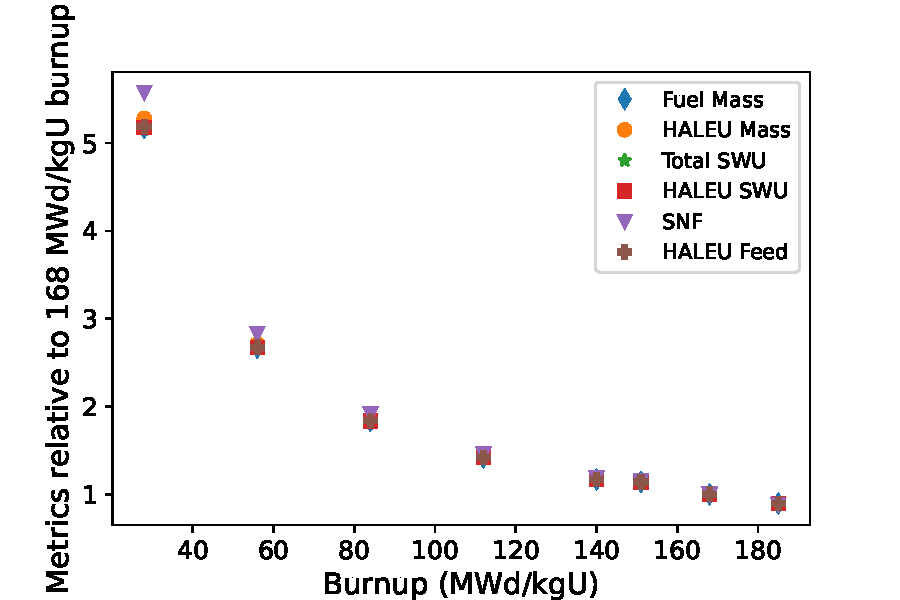
\includegraphics[scale=0.8]{xe100_bu.pdf}
    \caption{Change in metrics from varying the burnup of fuel 
    discharged from Xe-100, relative to a burnup of 168 MWd/kgU.}
    \label{fig:xe100_bu_s7}
\end{figure}

\subsection{MMR burnup}
When varying the \gls{MMR} discharge burnup, all of the metrics decrease, similar 
to what was observed by varying the Xe-100 discharge burnup, as shown in 
Figure \ref{fig:mmr_bu_s7}. One difference in 
the trends observed between varying these two parameters is the magnitude of 
the relative changes. Varying the \gls{MMR} burnup has a smaller relative effect 
on the metrics than varying the Xe-100 burnup because the \glspl{MMR}
meet a much smaller portion of the energy demand than the Xe-100s.
Therefore the impact on the cumulative metrics 
(what is reported here) is smaller. Another difference is that the total 
\gls{SWU}, \gls{HALEU} \gls{SWU}, and \gls{HALEU} feed increase the most 
when the \gls{MMR} burnup is low, compared with the \gls{UNF} having the 
greatest relative increase with the Xe-100 burnup is low. The difference 
in the relative change in \gls{UNF} is a result of the long cycle 
time of the \gls{MMR} and the results not accounting for 
\gls{UNF} still in a reactor at the end of the simulation, 
as previously discussed. 

\begin{figure}[h!]
    \centering
    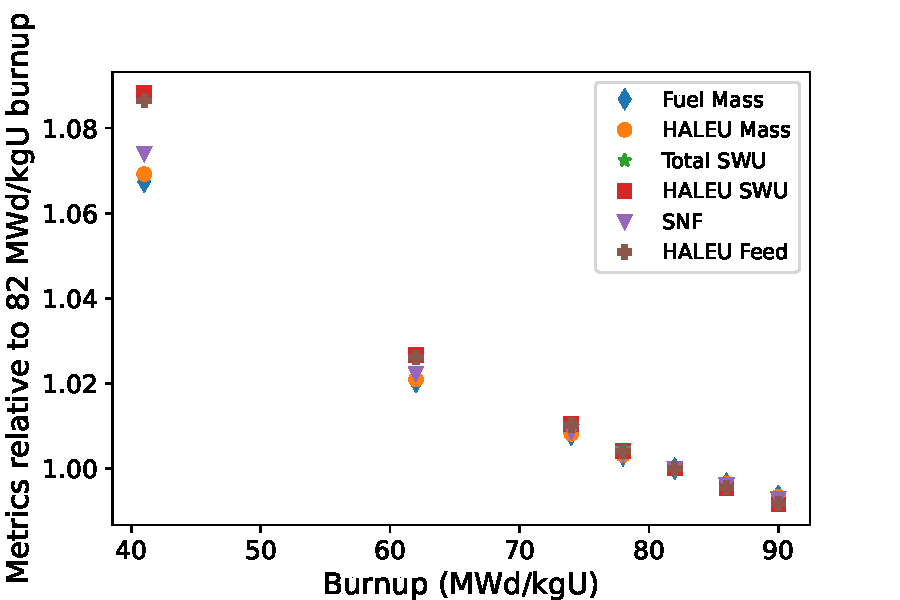
\includegraphics[scale=0.8]{mmr_bu.pdf}
    \caption{Change in metrics from varying the burnup of fuel 
    discharged from the MMR, relative to a burnup of 82 MWd/kgU.}
    \label{fig:mmr_bu_s7}
\end{figure}

\subsection{Burnup variations with a common build share}
To better investigate the effect of varying the discharge burnup of the Xe-100 
and \gls{MMR} without the influence of the deployment scheme preferentially
deploying Xe-100s, we repeated each set of analysis using a constant 20\% 
build share for both the Xe-100 and \gls{MMR} (VOYGRs meet the remaining 60\%). 
Using a constant build share for 
both reactors means that they each will supply the same fraction of the energy demand.
However, because of the different power output for each reactor a constant build 
share does not mean that the same number of each reactor is built. 

Figure \ref{fig:bu_constant} shows the relative change in each metric as a result 
of varying the \gls{MMR} (Figure \ref{fig:mmr_bu_constant}) and Xe-100 
(Figure \ref{fig:xe100_bu_constant}) discharge burnup with the constant build 
share. Changing the \gls{MMR} burnup has a greater impact with the specified 20\% 
build share than when the build share was not specified. This change is because 
more \glspl{MMR} are deployed with a 20\% build share than when the build share is 
not specified. Conversely, the Xe-100 burnup has a smaller impact on the metrics 
with a 20\% build share than when a build share isn't specified because fewer 
Xe-100s are deployed. 

\begin{figure}[h!]
    \centering
    \begin{subfigure}{0.48\textwidth}
        \centering
        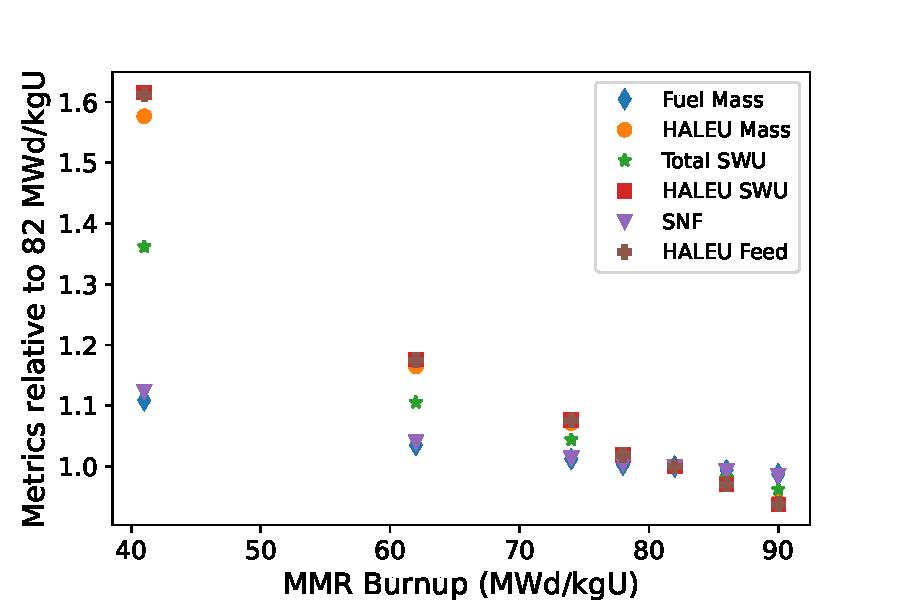
\includegraphics[width=\textwidth]{mmr_bu_constant.pdf}
        \caption{Change in metrics when varying the MMR discharge burnup.}
        \label{fig:mmr_bu_constant}
    \end{subfigure}
    \hfill
    \begin{subfigure}{0.48\textwidth}
        \centering
        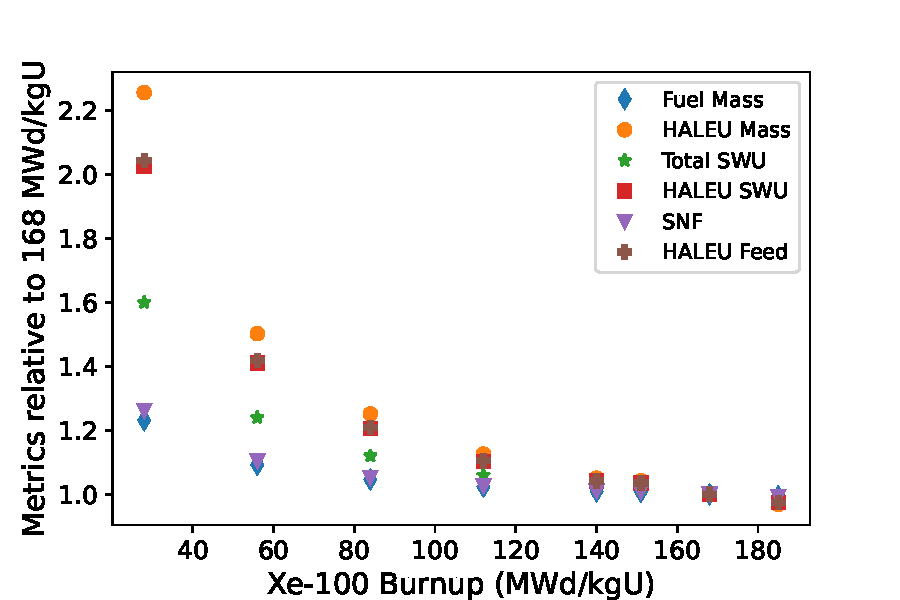
\includegraphics[width=\textwidth]{xe100_bu_constant.pdf}
        \caption{Change in metrics when varying the Xe-100 discharge burnup.}
        \label{fig:xe100_bu_constant}
    \end{subfigure}
    \caption{Relative changes in the metrics caused by changes in the discharge 
    burnup of the HALEU-fueled advanced reactors, assuming a constant 
    20\% build share for the Xe-100 and MMR.}
    \label{fig:bu_constant}
\end{figure}

By applying a constant build share, variations in these parameters lead to 
more variation in the effect on the metrics than when a build share was not 
specified. In these scenarios, varying the discharge burnup of either reactor 
leads to the greatest impact on the \gls{HALEU}-related metrics while the  
total fuel mass and \gls{UNF} mass are affected the least. 
The \gls{HALEU}-related metrics are affected the most because most of the 
energy demand is met through VOYGRs, which do not require \gls{HALEU}. 
Small changes in the each of the \gls{HALEU}-related metrics led to larger 
relative changes because these two reactors drive the effects on the 
\gls{HALEU}-related metrics. Conversely, the total fuel mass and \gls{UNF} 
masses are affected less by changes in these parameters because the fuel 
and \gls{UNF} for the VOYGRs are constant and the Xe-100 and \gls{MMR} 
have less of an impact on these two metrics. 

\section{Synergistic}\label{sec:synergistic}
The synergistic analysis in this work varied two parameters at a time to 
investigate some of the combined effects of the input parameters. Synergistic 
sensitivity analysis helps to identify if the combined effect of two parameters 
has a greater impact on the metrics that when varying a single parameter. 
We ran synergistic 
analysis on all combinations of two input parameters studied in the \gls{OAT} 
analysis, except combinations of two reactor build shares. The
results presented here are only a small subsection of the analysis performed, 
with the remaining results in Appendix \ref{app:s7_synergistic}.

\subsection{LWR lifetime and VOYGR build share}
When the percent of \glspl{LWR} operating for 80 years and the VOYGR build share 
are varied, the results are consistent with the results from varying 
each of the parameters by themselves. The effect on the \gls{HALEU} mass 
(Figure \ref{fig:lwr_voygr_share_enr_u}) is fairly uniform across the 
parameter space. As the VOYGR build share and percent of \gls{LWR} with 
extended licenses increase, the \gls{HALEU} mass required decreases, 
which is consistent with the results of the \gls{OAT} analysis for these 
parameters. By combining these two parameters, there is a greater 
decrease in the \gls{HALEU} mass than the decrease observed by just varying 
a single parameter. However, the linear trend in the metric
are consistent with the results of the \gls{OAT} analysis for 
each of these parameters, which suggests that these parameters do not 
interact with each other to cause a greater effect on the metric. 
The other \gls{HALEU} metrics, the \gls{HALEU} \gls{SWU} 
and \gls{HALEU} feed, also decrease in a similar manner as the \gls{HALEU} mass. 

\begin{figure}[ht]
    \centering
    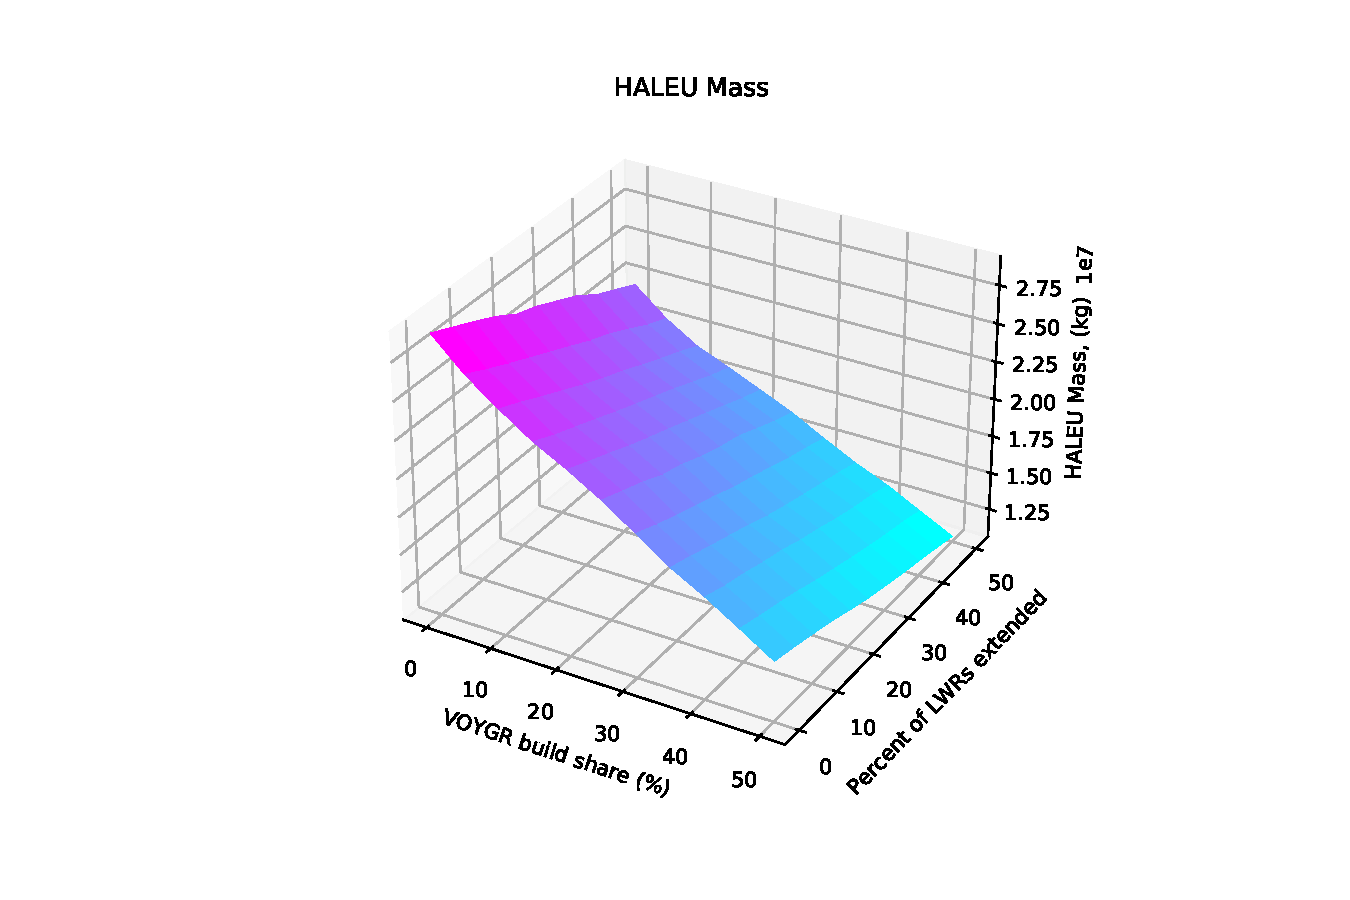
\includegraphics[scale=0.7,trim=120 0 120 30, clip]{lwr_voygr_share_haleu.pdf}
    \caption{Effect of the LWR lifetime and VOYGR build share on the HALEU mass.}
    \label{fig:lwr_voygr_share_haleu}
\end{figure}

The total enriched uranium mass decreases with increasing \gls{LWR} 
lifetimes, but increases with increasing VOYGR build share. There is a 
greater decrease in the total fuel mass required as the \gls{LWR} 
lifetime increases for greater values of VOYGR build share. This 
suggests some interaction between these two parameters on this 
output metric because the effects are not uniform across the parameter 
space. 

\begin{figure}[ht]
    \centering
    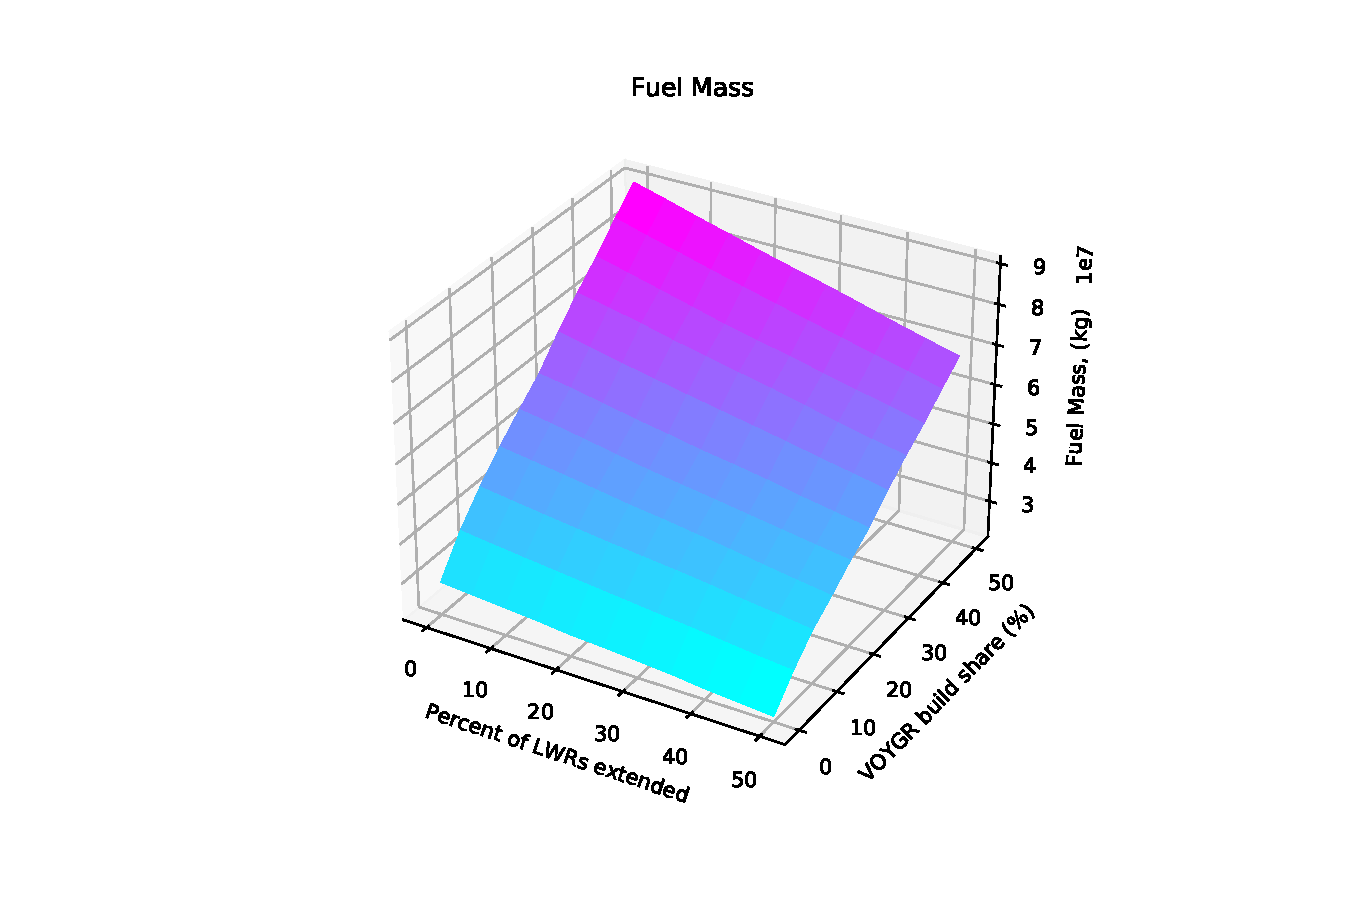
\includegraphics[scale=0.7,trim=120 0 120 30, clip]{lwr_voygr_share_enr_u.pdf}
    \caption{Effect of the LWR lifetime and VOYGR build share on 
    the total enriched uranium mass.}
    \label{fig:lwr_voygr_share_enr_u}
\end{figure}

\subsection{Xe-100 build share and Xe-100 burnup}
When the Xe-100 build share and discharge burnup are varied together,
there is a strong combined effect on the metrics. The \gls{HALEU} 
mass required (Figure \ref{fig:xe100_share_xe100_burnup_haleu}) 
increases as the burnup decreases and as the Xe-100 share increases.
The combined effect of these parameters is pronounced, such that there 
is a large increase in the \gls{HALEU} mass as the Xe-100 burnup 
reaches its minimum and the Xe-100 build share reaches its maximum. This 
effect stems from a larger portion of the advanced reactor fleet 
using its fuel less efficiently as this corner of the input space is 
reached. This result suggests that the discharge burnup of an advanced 
reactor should be considered when determining the build share of a reactor
type, if this metric is important. 

\begin{figure}[h!]
    \centering
    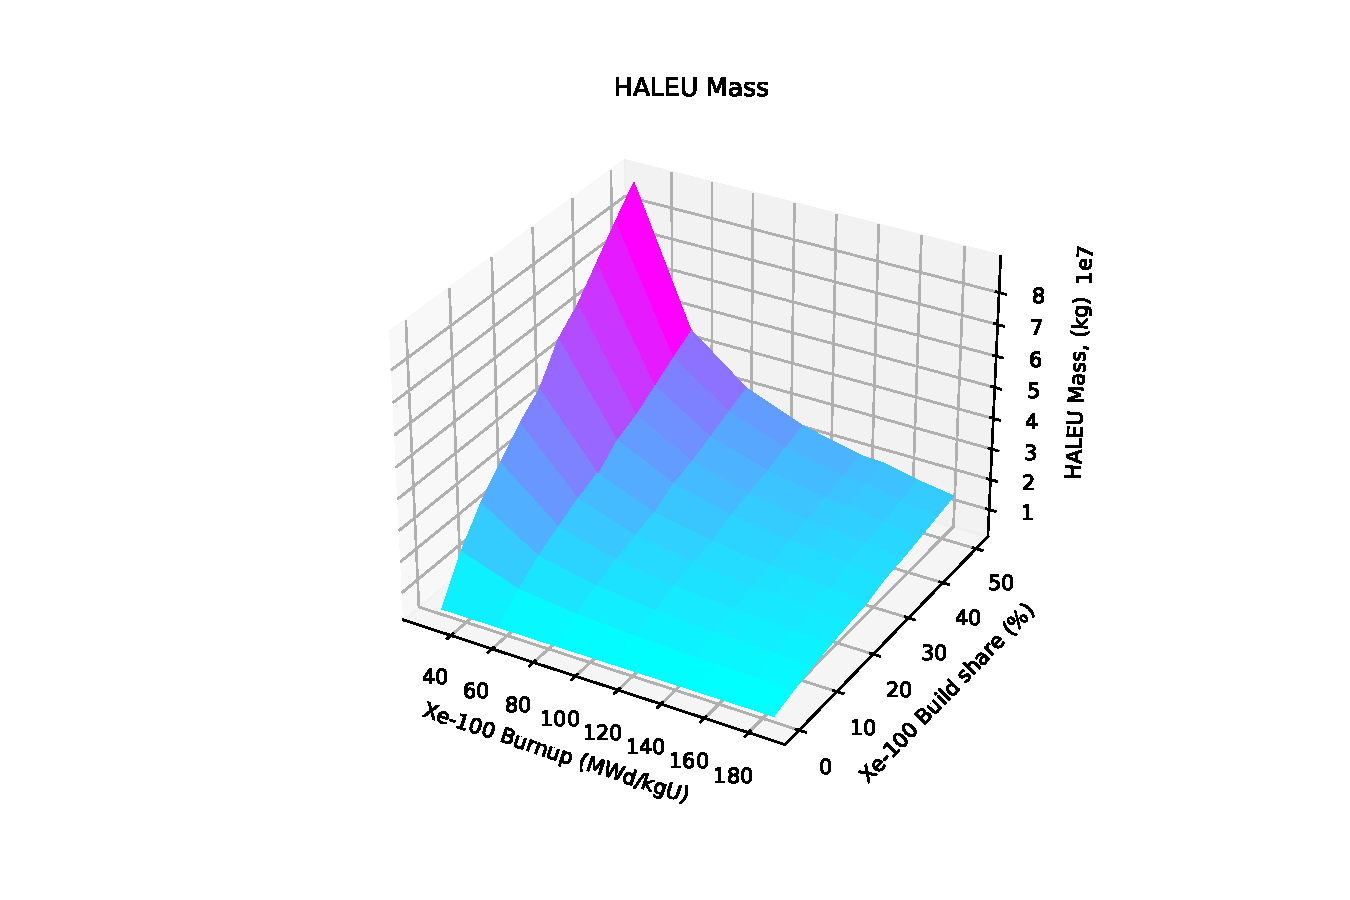
\includegraphics[scale=0.7, trim=120 0 120 30, clip]{xe100_share_xe100_burnup_haleu.pdf}
    \caption{Effect of Xe-100 discharge burnup and Xe-100 build share 
    on HALEU mass.}
    \label{fig:xe100_share_xe100_burnup_haleu}
\end{figure}

The total fuel mass (shown in Figure \ref{fig:xe100_share_xe100_burnup_enr_u})
reaches a minimum with a maximum Xe-100 build share 
and Xe-100 discharge burnup, which matches the trends observed in the 
\gls{OAT} analysis. A minimum is reached in this corner of the parameter 
space because more of the advanced reactor fleet is getting more 
energy out of the fuel used, so less fuel is required. Variations in the 
Xe-100 burnup do not affect the results when there is a 0\% Xe-100 build 
share because no Xe-100s are deployed. The Xe-100 build share does not 
greatly affect the fuel mass required when the Xe-100 has a discharge 
burnup of 28 MWd/kgU (the lowest value used in this work) because at this 
burnup level, the Xe-100 requires a similar amount of enriched uranium as 
the VOYGR for each 18 month period. Therefore, as the VOYGRs are replaced 
with Xe-100s, from increasing the Xe-100 build share, the cumulative total 
fuel mass required does not change much. 

\begin{figure}[h!]
    \centering
    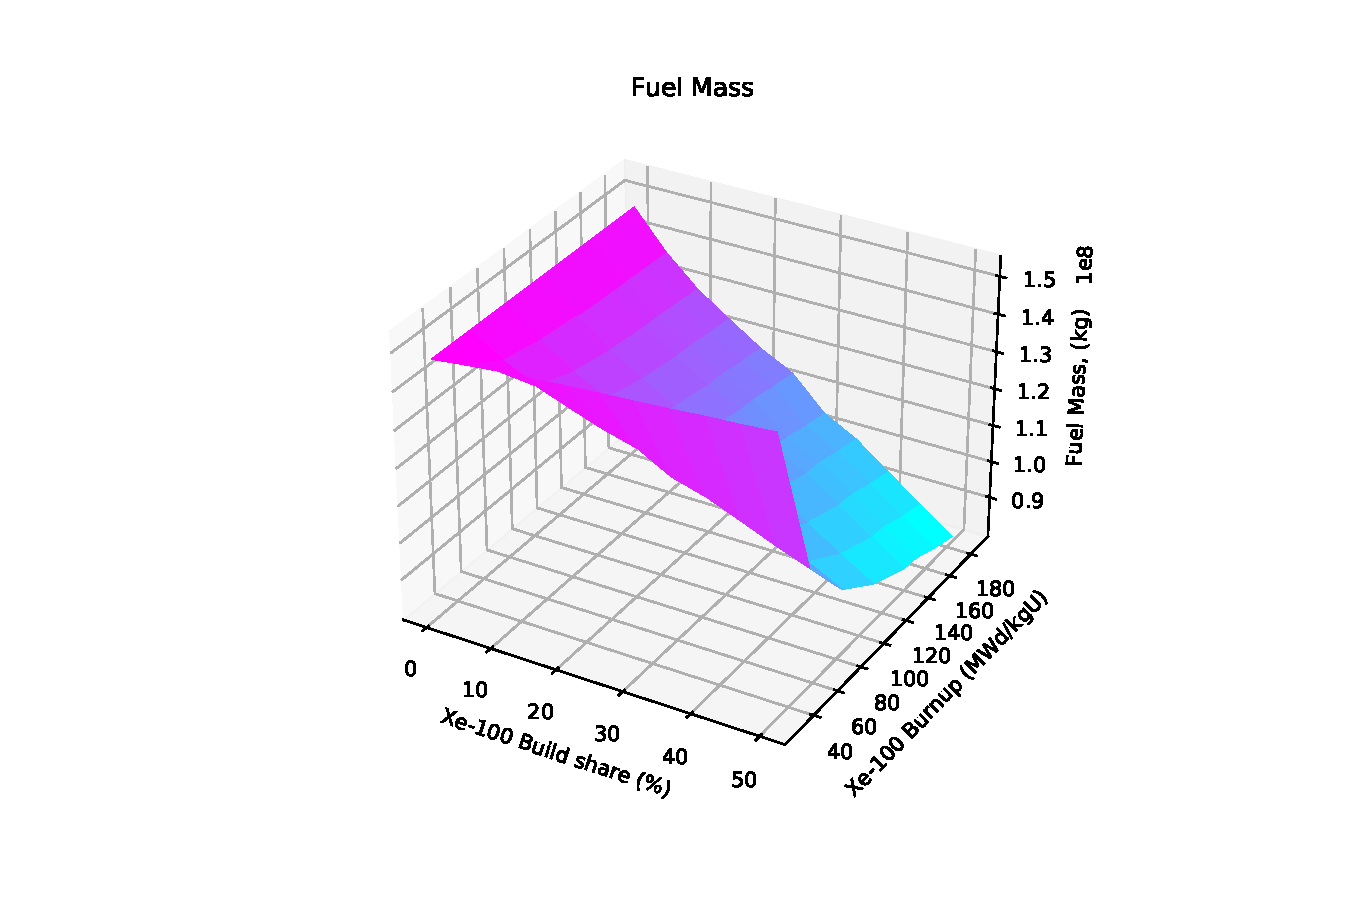
\includegraphics[scale=0.7, trim=120 0 120 30, clip]{xe100_share_xe100_burnup_enr_u.pdf}
    \caption{Effect of xe-100 discharge burnup and Xe-100 build share 
    on total fuel mass.}
    \label{fig:xe100_share_xe100_burnup_enr_u}
\end{figure}

\subsection{MMR build share and Xe-100 burnup}
When the \gls{MMR} build share and Xe-100 burnup are varied together, 
the effect on the metrics is not as consistent as the results from varying 
other pairs of parameters. As the Xe-100 burnup increases, the fuel mass 
decreases. However, the effect of increasing the \gls{MMR} build share 
is dependent on the Xe-100 discharge burnup. At smaller Xe-100 discharge 
burnup values, the fuel mass decreases with increasing \gls{MMR} build share. 
But at larger Xe-100 discharge burnup values, the fuel mass increases 
with increasing \gls{MMR} build share. The different trends result from 
changes in how much fuel the Xe-100 requires at each refueling and 
the difference between that and the amount of fuel required by the \gls{MMR}.
At the lowest burnup values, the Xe-100 requires more fuel than the 
\gls{MMR}. Therefore, as the Xe-100s are replaced with \glspl{MMR} from 
increasing the \gls{MMR} share, the 
total mass of fuel required in the transition decreases. However, as 
the Xe-100 burnup increases, the Xe-100 requires less fuel than the 
\gls{MMR}. Therefore, requiring more of the advanced reactor fleet to be 
\glspl{MMR} increases the total fuel mass required by advanced reactors in 
the transition. These results highlight how these two fuel cycle parameters 
interact to affect the output metrics. This pattern of results is observed 
for all six metrics considered in this work. 

\begin{figure}[h!]
    \centering
    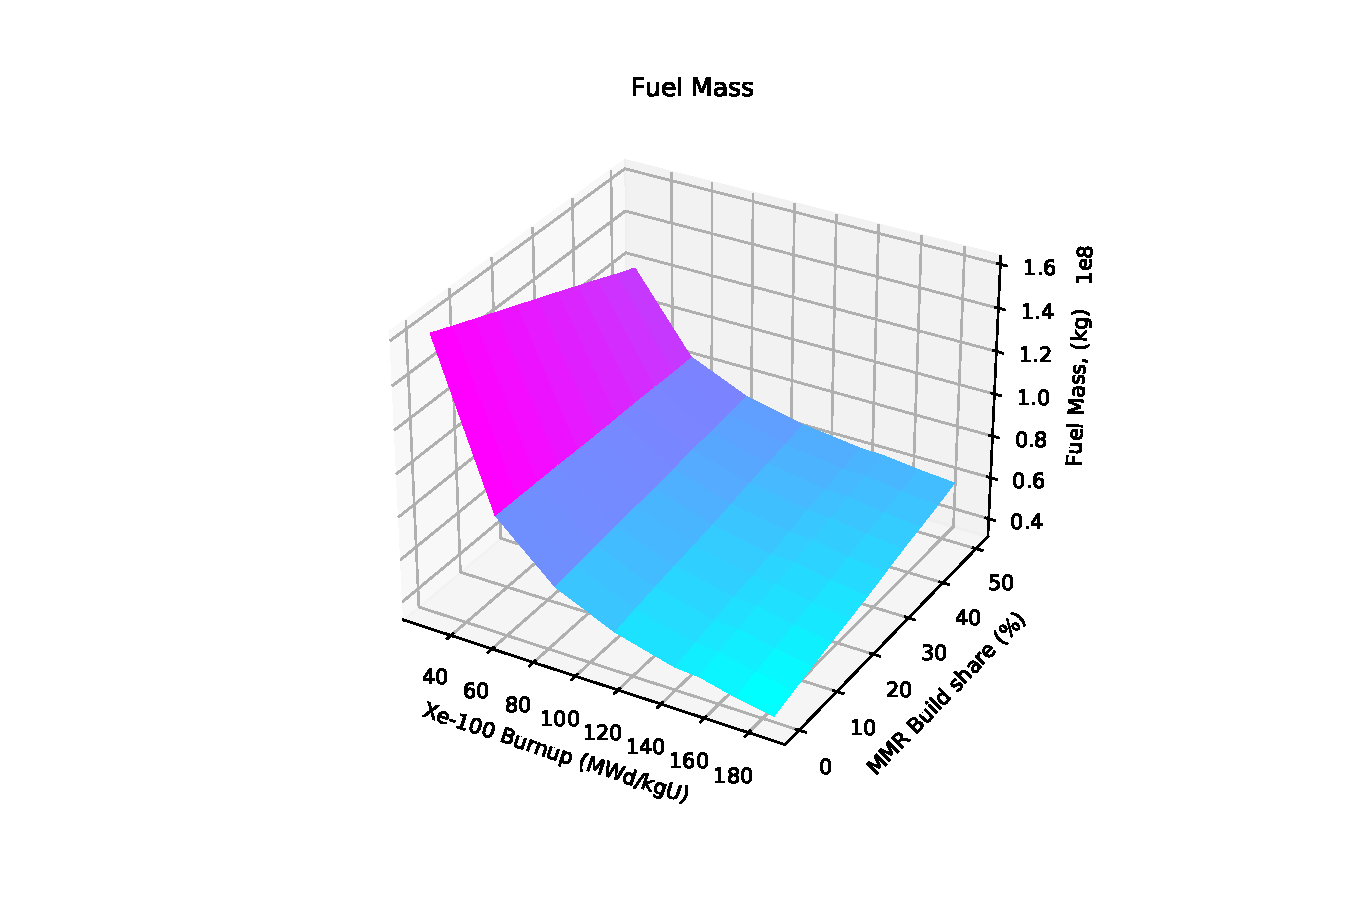
\includegraphics[scale=0.7, trim=120 0 120 30, clip]{mmr_share_xe100_burnup_enr_u.pdf}
    \caption{Effect of xe-100 discharge burnup and MMR build share 
    on total fuel mass.}
    \label{fig:mmr_share_xe100_burnup_enr_u}
\end{figure}


\subsection{Transition start and Xe-100 build share}
As Figure \ref{fig:ts_xe100_share_enr_u} shows, as the Xe-100 build 
share increases, the total fuel mass decreases. However, there is little 
effect in the total fuel mass as the transition start time is delayed 
because the magnitude of the effect on the fuel mass 
from varying the Xe-100 build share is greater than the magnitude of 
the effect from varying the transition start time. This is consistent 
with the results from the \gls{OAT} analysis, and is observed for five 
of the metrics considered in this work. This result suggests that the 
transition start time is not as important as the other parameters when 
trying to minimize or maximize certain metrics. 

\begin{figure}[h!]
    \centering
    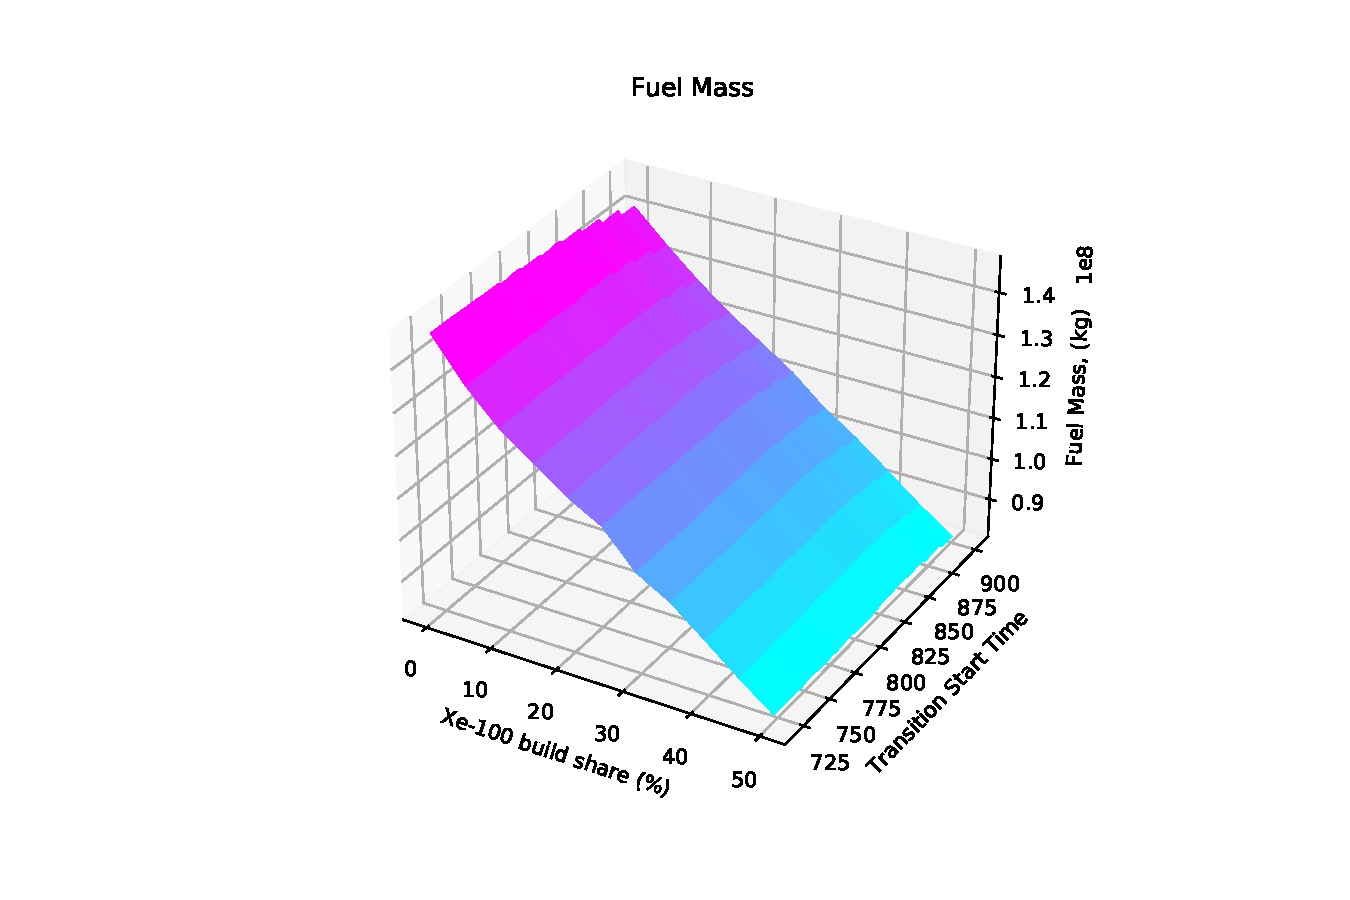
\includegraphics[scale=0.7, trim=120 0 120 0, clip]{ts_xe100_share_enr_u.pdf}
    \caption{Effect of transition start time and Xe-100 build share 
    on total fuel mass.}
    \label{fig:ts_xe100_share_enr_u}
\end{figure}

The effect of varying these two parameters is the opposite when the total 
\gls{SWU} capacity is considered: varying the transition start time has 
a greater impact on the metric than varying the Xe-100 build share. This 
result stems from the similar \gls{SWU} capacities needed for the Xe-100 
and VOYGR leading to little change in the total \gls{SWU} capacity when 
varying the Xe-100 build share. Therefore, the transition start time has 
more impact on this metric than the Xe-100 build share, and there is little 
of a combined effect observed because of the small impact from each parameter 
on this metric. 

\begin{figure}[h!]
    \centering
    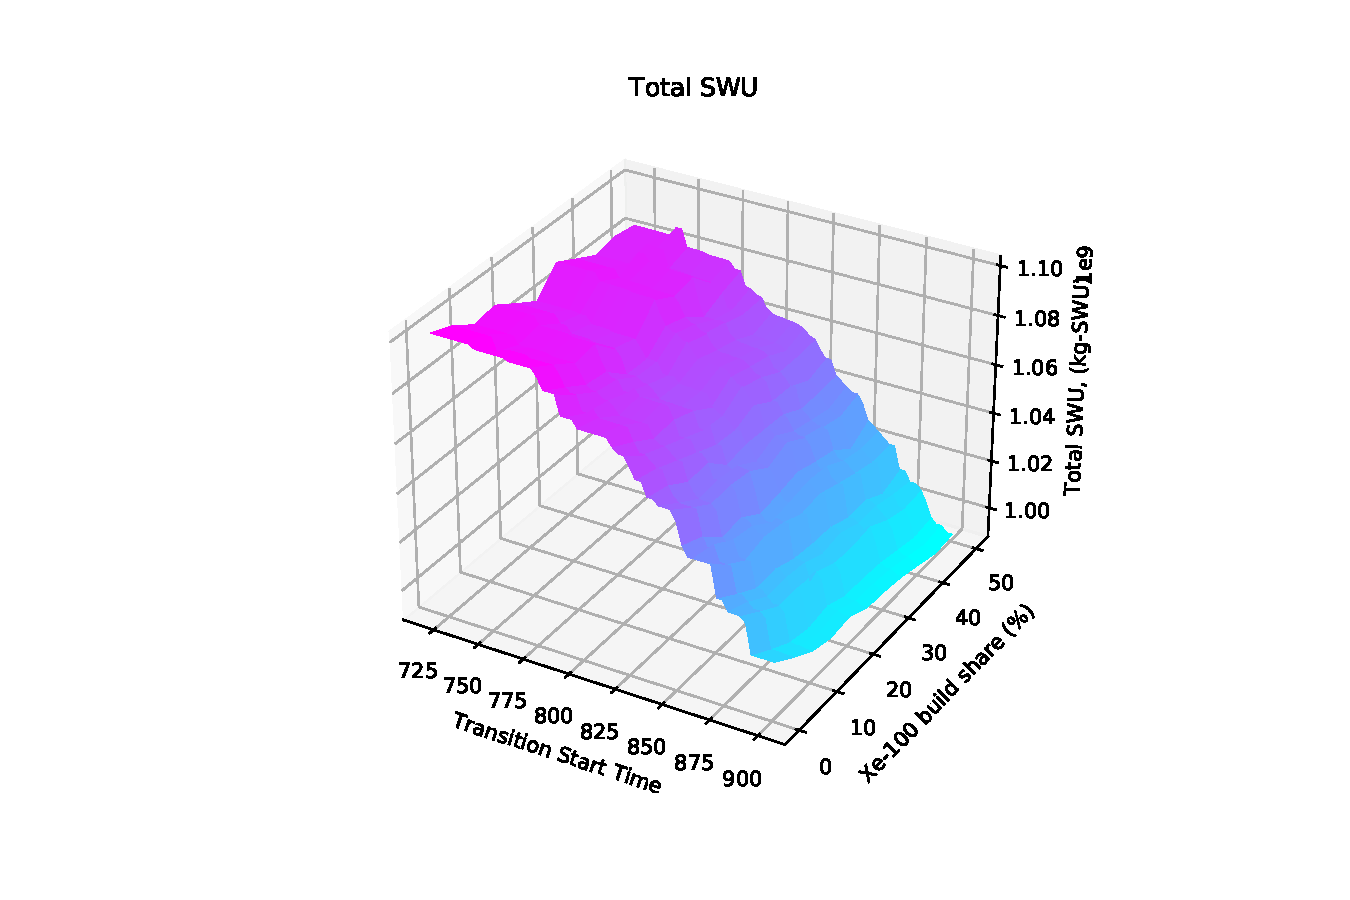
\includegraphics[scale=0.7, trim=120 0 120 0, clip]{ts_xe100_share_swu.pdf}
    \caption{Effect of transition start time and Xe-100 build share 
    on total fuel mass.}
    \label{fig:ts_xe100_share_swu}
\end{figure}

\section{Global}
In each calculation of the global sensitivity analysis, we varied 
the transition start 
time, percent of \glspl{LWR} operating for 80 years, the Xe-100 discharge 
burnup, \gls{MMR} burnup, and build share of one advanced reactor. 
We decided to perform this analysis three separate times instead of 
varying all seven variables to prevent unwanted combinations of the 
advanced reactor build shares that result in an oversupply or 
undersupply of power. 

Instead of comparing ranges and values of each metric in this 
analysis, we compared the variance each input parameter causes in 
the output metrics through the Sobol' indices. 
To assist in calculating the Sobol' indices, we created surrogate 
models for each of the iterations. These models are approximations 
of the relationships between the input and output parameters,
are computationally inexpensive \cite{adams_dakota_2021}, and 
assist in exploring an entire input space, as compared with 
exploring an input space in a grid search. To generate 
each of the surrogate models (one for each advanced reactor build share 
variation), we ran 4000 different fuel cycle transitions based on guidance 
from the Dakota manual \cite{adams_dakota_2021} to run 

\begin{equation}
    100\times P\times(R+2)
    \label{eq:surrogate}
\end{equation}

\noindent number of cases to build the surrogate model 
In Eq \ref{eq:surrogate}, $P$ is the number of input parameters and 
$R$ is the number out response metrics. 

In each of these
transitions, we allowed most of the input parameters vary freely 
within a given range (defined in Table \ref{tab:global_ranges}), 
and used Latin Hypercube Sampling (a near-random technique in 
Dakota) to select parameter values. We did not allow 
the Xe-100 discharge burnup to vary freely within a range 
when running the initial transition scenarios. We kept this input
parameter constrained to 
specific values, like in the \gls{OAT} analysis. The burnup values 
considered for the sensitivity 
analysis thus far are based on integer numbers of passes through 
the core (batches) and integer number of 
months for the cycle lengths of this reactor. By using 
Xe-100 burnup values that correspond to integer values, we can 
adhere to the integer value restrictions in \Cyclus on the number of 
batches in a core.
We expanded the Xe-100 discharge burnup values considered 
to provide additional data points off of which to 
generate the surrogate model. We selected additional burnup points 
to represent 
between one and six passes for each pebble with a residence time of six, seven, 
or eight months for each pass. This expansion of the Xe-100 burnup resulted 
in 16 different burnup values between 28-185 MWd/kgU.
We converted the \gls{MMR} burnup 
from a discrete variable to a continuous variable by varying 
the lifetime of the reactor as need to achieve the burnup value. We made 
this conversion from discrete to continuous for the \gls{MMR} burnup 
because the lack of multiple batches in the core means that there are 
no inherent restrictions to integer numbers. 

\begin{table}[h!]
    \centering 
    \caption{Ranges of the input parameters considered for generating 
    surrogate models in the global sensitivity analysis. The Xe-100 
    burnup was constrained to 16 different values within the given range, 
    while the other variables were free to vary within the defined range.}
    \label{tab:global_ranges}
    \begin{tabular}{c c c}
        \hline
        Input parameter & Range & Units \\
        \hline 
        Transition start time & January 2025-January 2040 & - \\
        LWR lifetime extensions & 0-50 & \% \\
        Reactor build share & 0-50 & \% \\
        \gls{MMR} burnup & 41-90 & MWd/kg \\
        Xe-100 burnup & 28-185 & MWd/kg \\
        \hline
    \end{tabular}
\end{table}

After explicitly modeling the transition scenarios with different 
combinations and the specific Xe-100 burnup values, we 
created surrogate models. 
When creating the surrogate model, we once again used the Latin Hypercube 
sampling 
for all of the variables, but allowed all of the input parameters to be 
continuous variables. The surrogate models are not bound by 
the variable-type restriction in \Cyclus, so we were able to allow 
the Xe-100 burnup to not be bound by integer numbers of batches. 
We used both the quadratic and Gaussian fits to the data 
to create the surrogate models, similar to what Richards and 
Feng did \cite{richards_application_2021}. The quadratic method defines a 
second-order response surface based on linear least squares regressions methods 
\cite{adams_dakota_2021}. The Gaussian method uses a Gaussian correlation function 
to define a response surface \cite{adams_dakota_2021}. We used both methods were 
used to provide a comparison of the different methods, since they each have
limitations. 
The quadratic method does not implement any forward- or backward-stepping regression 
methods to remove unnecessary terms in the polynomial fit, and the Gaussian method 
may discard points if the data points are poorly spaced \cite{adams_dakota_2021}.
These limitations in the methods contributed to the decision to have as many 
input parameter data points as possible. 
We also instructed Dakota to perform variance decomposition 
on both of the surrogate models to calculate the Sobol' indices.

The results presented in this section include the results from the initial 
transitions modeled, the results from the surrogate models, and the Sobol' indices 
that describes the impact of each input parameter on each output metric. The 
results from the modeled transitions and the surrogate models provide 
information of how well the surrogate models fit some of the trends and 
relationships 
between the input parameters and output metrics. 
The total and the main Sobol' indices reported describe the contribution 
from each parameter and its interactions with all of the other parameters 
and the contribution from each individual parameter, respectively. 

\subsection{Xe-100 build share}
This section provides the results of the global sensitivity analysis using 
both a Gaussian and a quadratic surrogate model when varying the Xe-100 build 
share. 

\subsubsection{Gaussian surrogate model}
The Gaussian surrogate model for the variations in the Xe-100 build 
share results in an R$^2$ value of 1 for each metric. This value 
means that the outputs of 
the surrogate model match perfectly to the data provided from the initial 
\Cyclus runs. The large R$^2$ value suggests that this surrogate model type 
fits to noise in the data provided. 
Figure \ref{fig:s7_xe100_gaussian} compares the values of the
\gls{HALEU} mass as a function of the Xe-100 burnup for the Gaussian model 
and the input data (the explicitly modeled transitions). The results of 
the Gaussian model follows the input 
data well, nearly reaching the maximum and minimums of the data. However, 
closer inspection of the data shows that results of the Gaussian model 
include non-physical results, such as negative values of \gls{HALEU} mass. 
These values suggest that the Gaussian model extrapolates to obtain 
some of the values, instead 
of just interpolating. Therefore, the Gaussian model is not a perfect 
match to the input data, which means that the Sobol' indices are different 
than if the variance decomposition were performed directly on the input 
data. 

\begin{figure}[h!]
    \centering 
    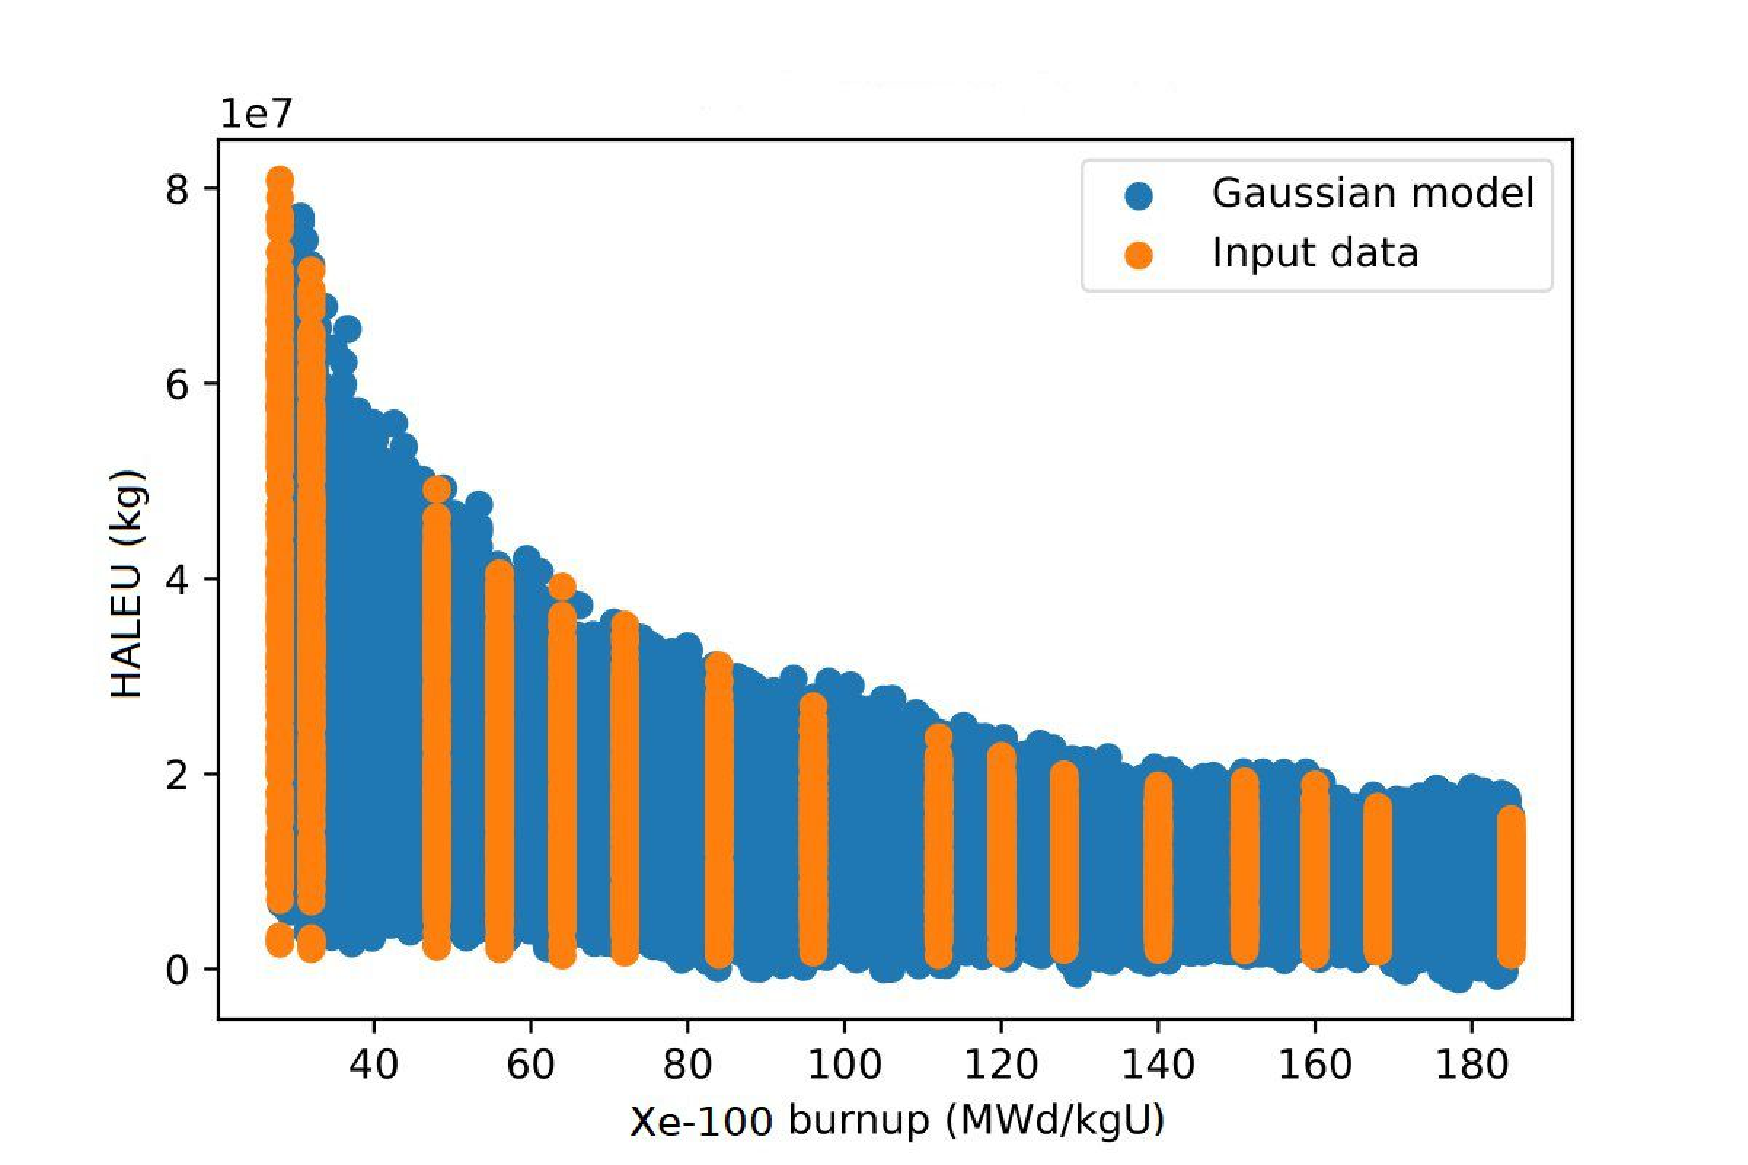
\includegraphics[scale=0.8]{xe100_share_gaussian_xe100_burnup_haleu.pdf}
    \caption{Comparison of the input data and the results of the Gaussian 
    surrogate model when the Xe-100 build share is varied.}
    \label{fig:s7_xe100_gaussian}
\end{figure}

Table \ref{tab:s7_sobol_xe100_gaussian} reports the main and total Sobol' indices 
for each input parameter on each output metric. The highlighted cells have 
a total Sobol' index of at least 0.5, to indicate parameters that have a large 
effect on the metrics. 
The transition start time 
has little effect on any of the metrics, which is consistent with the 
results of the \gls{OAT} and synergistic analysis. The \gls{LWR} lifetimes 
do not greatly affect any of the \gls{HALEU}-related metrics or the 
total \gls{SWU} capacity because this parameter primarily delays when 
the \gls{HALEU}-fueled reactors are deployed and not how many are deployed. 
The \gls{LWR} lifetimes have some impact on the total 
fuel mass and the \gls{SNF} mass, but less of an impact than the Xe-100 
build share. 
The \gls{MMR} burnup has a small Sobol' index for all of the output metrics
because a very small portion of the fleet are \glspl{MMR}. 

The Xe-100 build share and burnup have a large effect (total Sobol' indices 
more than 0.5) on all three of the \gls{HALEU}-related metrics because the 
number of \glspl{MMR} built in these transitions are relatively constant and the 
variations in the Xe-100s drive the changes in these metrics. The Xe-100 build share 
does not have as much of an impact on the total \gls{SWU} capacity because 
of the similar \gls{SWU} capacity required by the Xe-100 and the VOYGR and 
the replacement of VOYGRs with Xe-100s as the Xe-100 build share increases. 
The Xe-100 build share has the largest impact on the total fuel mass 
and the \gls{SNF} mass because 
of the replacement of Xe-100s with VOYGRs as the Xe-100 build share decreases and 
the large difference in fuel mass required by these two reactors. The Xe-100 
burnup has the largest impact on the total \gls{SWU} capacity because as this 
parameter varies, so does the difference in \gls{SWU} capacity needed to fuel the Xe-100 
and the \gls{SWU} capacity needed to fuel the VOYGR.

\begin{table}[h!]
    \centering
    \caption{Sobol' indices for the Gaussian model when varying the 
    Xe-100 build share. The first value is the 
    main index, the second value is the total index. Highlighted 
    values indicate a total Sobol' indices of above 0.5.}
    \label{tab:s7_sobol_xe100_gaussian}
    \begin{tabular}{c c c c c c c}
        \hline
        & \multicolumn{6}{c}{Output Metric} \\
        Parameter & Fuel Mass & HALEU Mass & SWU & HALEU SWU & Feed & SNF Mass \\
        \hline
        Transition Start & 0.003/0.003 & 0.007/0.007 & 0.007/0.009 &
                           0.009/0.009 & 0.006/0.009 & 0.003/0.003\\
        LWR Lifetime & 0.268/0.280 & 0.012/0.021 & 0.081/0.095 &
                       0.013/0.022 & 0.013/0.022 & 0.301/0.314\\
        Xe-100 Build Share & \cellcolor{green!25}0.478/0.533 & \cellcolor{green!25}0.375/0.513 & 0.099/0.283 &
        \cellcolor{green!25}0.374/0.511 & \cellcolor{green!25}0.374/0.512 & 0.411/0.474\\
        Xe-100 Burnup & 0.188/0.247 & \cellcolor{green!25}0.465/0.571 & \cellcolor{green!25}0.622/0.775 & 
        \cellcolor{green!25}0.463/0.568 & \cellcolor{green!25}0.463/0.568 & 0.214/0.280\\
        MMR Burnup & 0.002/0.002 & 0.003/0.004 & 0.005/0.006 & 
                     0.004/0.005 & 0.004/0.005 & 0.002/0.002\\
        \hline        
    \end{tabular}
\end{table}

\subsubsection{Quadratic surrogate model}
When using a quadratic surrogate model, the R$^2$ values for the training points on 
each output metric range between 0.921-0.966. Therefore, these model are  
expected to 
fit the input data provided but not be fit to the noise in the input data 
as much as the Gaussian model. A comparison of the Xe-100 burnup and \gls{HALEU} 
mass for the input data and the results of the quadratic model (Figure 
\ref{fig:s7_xe100_quadratic}) shows that the quadratic model does 
capture the overall trend of the input data. However, like the Gaussian model, 
the quadratic model gives the non-physical result of a negative \gls{HALEU} mass
at some points. Additionally, 
the results of the quadratic model do not meet the maximum of the input data and 
provide multiple results below the minimum value of the input data. Therefore, 
the quadratic model is also performing some extrapolation of the data based on the 
fit placed on the data.

\begin{figure}[h!]
    \centering 
    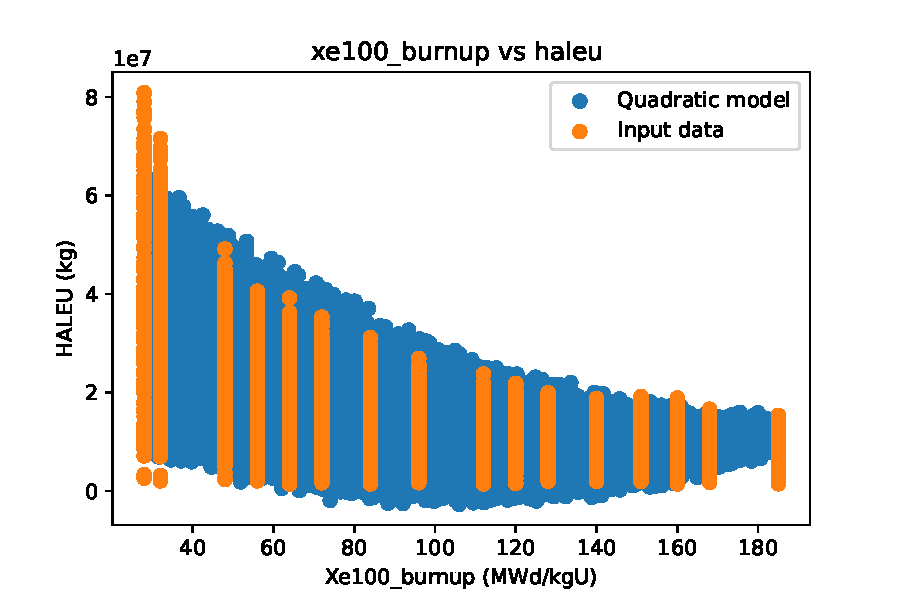
\includegraphics[scale=0.8]{xe100_share_quadratic_xe100_burnup_haleu.pdf}
    \caption{Comparison of the input data and the results of the quadratic 
    surrogate model when the Xe-100 build share is varied.}
    \label{fig:s7_xe100_quadratic}
\end{figure}

Table \ref{tab:s7_sobol_xe100_quadratic} provides the main and total Sobol' 
indices for each of the input parameters on each output metric. The 
green cells identify total Sobol' indices that are at least 0.5. The same patterns 
observed in the Sobol' indices from the Gaussian model are 
observed in the values from the quadratic model as well. The Xe-100 build share 
and Xe-100 burnup affect the metrics the most, the \gls{LWR} lifetime has some 
impact, and the \gls{MMR} burnup and transition start time has the smallest impact 
on the metrics. 

\begin{table}[h!]
    \centering
    \caption{Sobol' indices for the quadratic model when varying the Xe-100 
    build share. The first number is the main index, the second is the total 
    index. Highlighted 
    values indicate a total Sobol' indices of above 0.5.}
    \label{tab:s7_sobol_xe100_quadratic}
    \begin{tabular}{c c c c c c c}
        \hline
        & \multicolumn{6}{c}{Output Metric} \\
        Parameter & Fuel Mass & HALEU Mass & SWU & HALEU SWU & Feed & SNF Mass \\
        \hline
        Transition Start & 0.000/0.000& 0.006/0.005 & 0.007/0.007 &
                           0.008/0.007 & 0.008/0.007 & 0.002/0.004\\
        LWR Lifetime & 0.278/0.286 & 0.014/0.021 & 0.082/0.089 & 
                       0.015/0.022 & 0.015/0.022 & 0.310/0.319\\
        Xe-100 Build Share & \cellcolor{green!25}0.443/0.501 & \cellcolor{green!25}0.374/0.500 & 0.115/0.283 & 
                             0.374/0.499 & 0.374/0.499 & 0.375/0.441\\
        Xe-100 Burnup & 0.214/0.279 & \cellcolor{green!25}0.472/0.578 & \cellcolor{green!25}0.624/0.773 &
                        \cellcolor{green!25}0.470/0.576 & \cellcolor{green!25}0.430/0.576 & 0.243/0.315\\
        MMR Burnup & 0.001/0.001 & 0.002/0.002 & 0.004/0.004 &
                     0.003/0.003 & 0.003/0.003 & 0.001/0.001\\
        \hline        
    \end{tabular}
\end{table}

The two surrogate models result in different Sobol' indices for each 
input parameter/output metric pair. These differences are likely a result 
of how the models fit the data. The Gaussian model fits 
better the the extremes and trends in the input data points and does not 
assume a specific form for the data, but the 
quadratic model does not fit to the noise in the input data as much. 
However, the two models are consistent in 
their relative comparison of how much each input parameter affects the output 
metrics, and are consistent with the results from the \gls{OAT} and 
synergistic analysis. The two models are also consistent in 
identifying that the Xe-100 build share and Xe-100 burnup 
have the largest impact on the metrics.

\subsection{MMR build share}
This section provides the results of the global sensitivity analysis using 
both a Gaussian and a quadratic surrogate model when varying the \gls{MMR} 
build share. 

\subsubsection{Gaussian surrogate model}
The Gaussian model has an R$^2$ value of 1 with respect to each of the output 
metrics. This value means that these models are also expected to fit the input 
data very well, including any noise present in the data. As Figure 
\ref{fig:s7_mmr_gaussian} shows, the data from the Gaussian model fits well 
to the input data provided. Unlike the models predicted based on input data when 
varying the Xe-100 build share, this model does not result in any negative 
mass values. However, it still results in mass values lower than what is 
present in the input data which suggests that this model also extrapolates 
on some of the data. It also does not fully predict some of the outliers in 
the data, such as the maximum \gls{HALEU} mass at a burnup at 128 MWd/kg.

\begin{figure}[h!]
    \centering 
    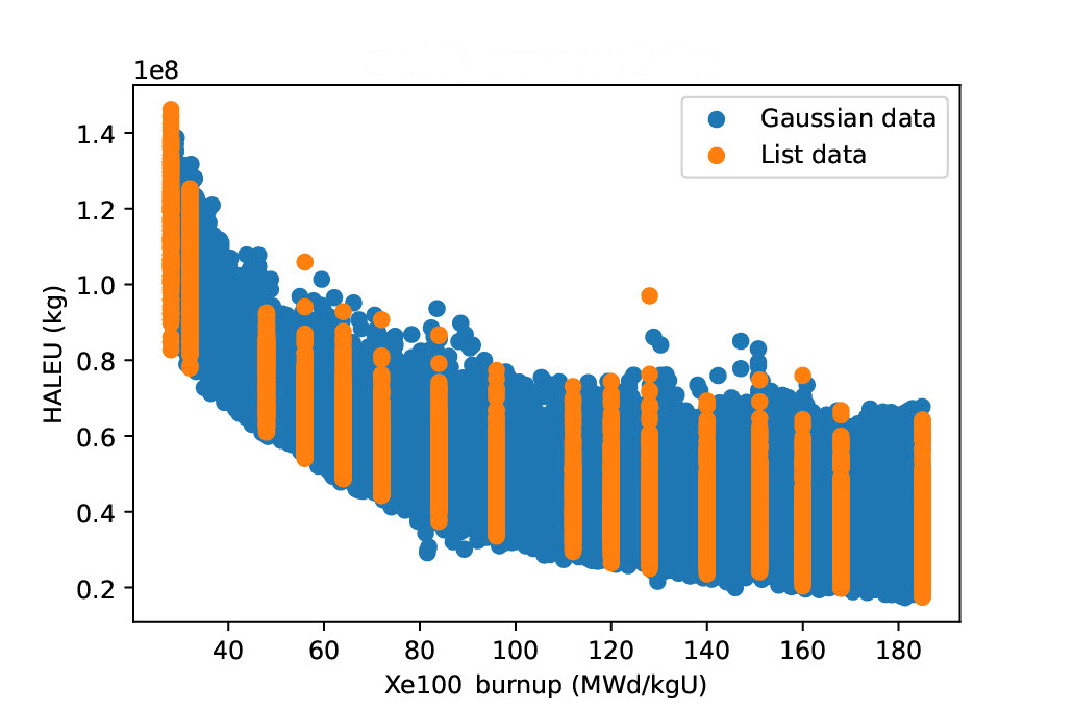
\includegraphics[scale=0.8]{mmr_share_gaussian_xe100_burnup_haleu.pdf}
    \caption{Comparison of the input data and the results of the Gaussian 
    surrogate model when varying the MMR build share.}
    \label{fig:s7_mmr_gaussian}
\end{figure}

Examination of the Sobol' indices for this model (Table \ref{tab:s7_sobol_mmr_gaussian})
shows that the Xe-100 burnup has the largest impact and a significant impact (i.e., 
total indices greater than 0.5) on all of the 
output metrics. One may expect the \gls{MMR} 
build share and \gls{MMR} burnup to have a strong combined impact on 
the results. However, this result is consistent with the results 
shown for the synergistic analysis (Figures \ref{fig:mmr_share_xe100_burnup} and 
\ref{fig:mmr_share_mmr_burnup}). When the Xe-100 burnup was varied in combination 
with the \gls{MMR} share, the range of values for each metric was larger than 
when the \gls{MMR} burnup was varied with the \gls{MMR} build share. Variations 
in the \gls{MMR} build share replaces Xe-100s with \glspl{MMR}. The variations 
in the Xe-100 burnup lead to greater changes in the metrics than variations 
in the \gls{MMR} burnup, as shown in Figure \ref{fig:bu_constant}, because 
the Xe-100 burnup values span a larger range and the compounding effects of the 
multiple batches in the Xe-100. 
Similar to the results from varying the Xe-100 build share, the 
transition start time has effectively no impact on the results. The \gls{LWR} 
lifetime has less of an impact on the metrics than when the Xe-100 
build share was varied. The \gls{MMR} burnup also has little impact on the 
output metrics. 

\begin{table}[h!]
    \centering
    \caption{Sobol' indices for the Gaussian model when varying the MMR 
    build share. The first number is the main index, the second is the total 
    index. Highlighted 
    values indicate a total Sobol' indices of above 0.5.}
    \label{tab:s7_sobol_mmr_gaussian}
    \begin{tabular}{c c c c c c c}
        \hline
        & \multicolumn{6}{c}{Output Metric} \\
        Parameter & Fuel Mass & HALEU Mass & SWU & HALEU SWU & Feed & SNF Mass \\
        \hline
        Transition Start & 0.001/0.006 & 0.000/0.004 & 0.001/0.001 &
                           0.001/0.001 & 0.001/0.001 & 0.001/0.006\\
        LWR Lifetime & 0.054/0.068 & 0.047/0.063 & 0.055/0.071 &
                       0.054/0.069 & 0.054/0.069 & 0.057/0.071\\
        MMR Build Share & 0.069/0.107 & 0.068/0.107 & 0.162/0.203 &
                          0.162/0.204 & 0.152/0.193 & 0.015/0.055\\
        Xe-100 Burnup & \cellcolor{green!25}0.806/0.846 & \cellcolor{green!25}0.819/0.858 & \cellcolor{green!25}0.700/0.732 &
        \cellcolor{green!25}0.701/0.734 & \cellcolor{green!25}0.713/0.747 & \cellcolor{green!25}0.858/0.900\\
        MMR Burnup & 0.035/0.049 & 0.037/0.050 & 0.054/0.071 &
                     0.054/0.071 & 0.052/0.069 & 0.038/0.053\\
        \hline        
    \end{tabular}
\end{table}

\subsubsection{Quadratic surrogate model}
When using the quadratic surrogate model, the model has an R$^2$ value of 0.94
with respect to each of the output metrics. Therefore, these models also fit 
the data well without fitting all of the noise present in the input data. 
As Figure \ref{fig:s7_mmr_quadratic} shows, the output of the quadratic model 
fits the input data well, but not perfectly. Similar to the quadratic 
model created from varying the Xe-100 build share, this model 
does not perform well in fitting the maximum values and under-predicts 
some of the minimum values in the input data. 

\begin{figure}[h!]
    \centering 
    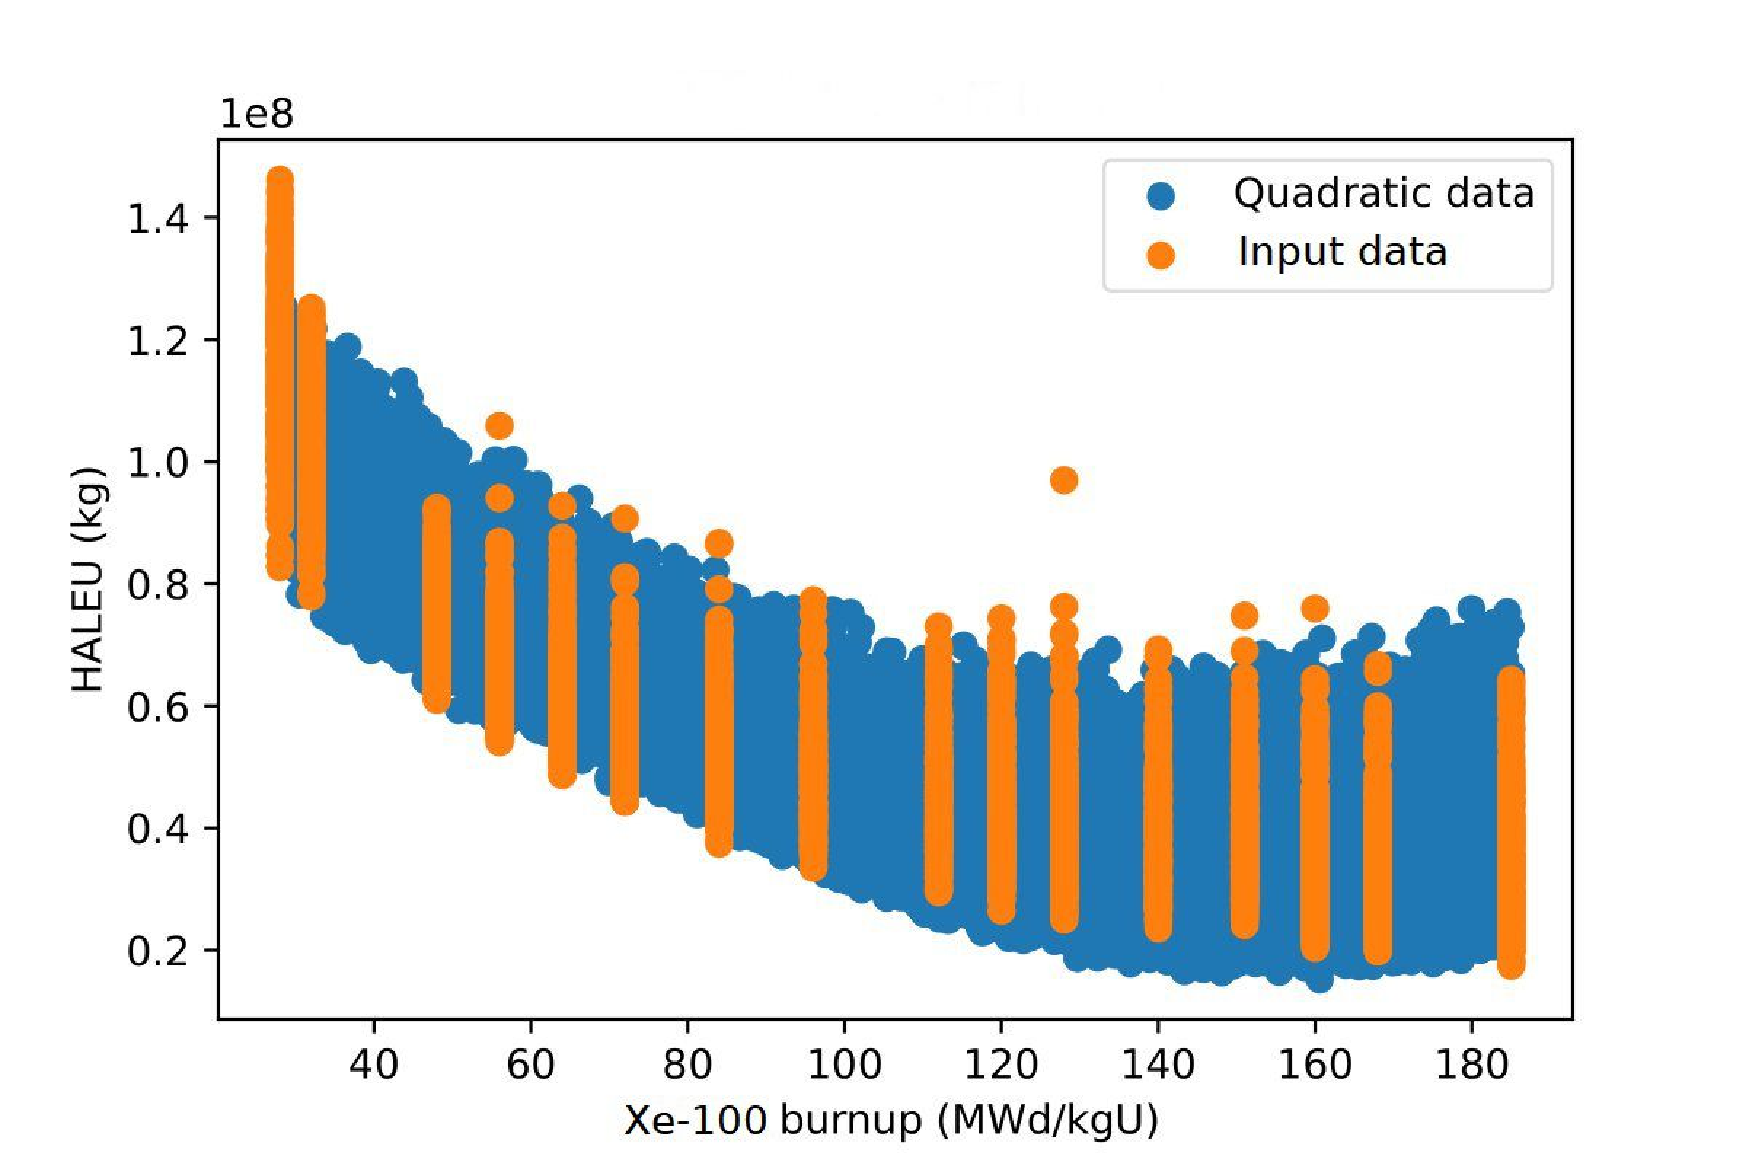
\includegraphics[scale=0.8]{mmr_share_quadratic_xe100_burnup_haleu.pdf}
    \caption{Comparison of the input data and the results of the quadratic 
    surrogate model when varying the MMR build share.}
    \label{fig:s7_mmr_quadratic}
\end{figure}

The Sobol' indices from the quadratic model (Table 
\ref{tab:s7_sobol_mmr_quadratic}) are similar to those from the 
Gaussian model. The Xe-100 burnup has the largest impact on all of the 
output metrics. The \gls{MMR} build share has the next largest impact 
on the metrics, but it is a very small impact. The other model 
parameters have a negligible effect on the metrics. The Sobol' 
indices from this model are very similar to those from the Gaussian 
model. 

\begin{table}[h!]
    \centering
    \caption{Sobol' indices for the quadratic model when varying the MMR 
    build share. The first number is the main index, the second is the total 
    index. Highlighted 
    values indicate a total Sobol' indices of above 0.5.}
    \label{tab:s7_sobol_mmr_quadratic}
    \begin{tabular}{c c c c c c c}
        \hline
        & \multicolumn{6}{c}{Output Metric} \\
        Parameter & Fuel Mass & HALEU Mass & SWU & HALEU SWU & Feed & SNF Mass \\
        \hline
        Transition Start & 0.002/0.003 & 0.000/0.000 & 0.000/0.000 &
                        0.000/0.000 & 0.000/0.000 & 0.002/0.003\\
        LWR Lifetime & 0.023/0.062 & 0.046/0.054 & 0.050/0.059 &
                       0.049/0.057 & 0.049/0.057 & 0.054/0.064\\
        MMR Build Share & 0.051/0.087 & 0.052/0.089 & 0.133/0.171 &
                          0.133/0.171 & 0.124/0.162 & 0.008/0.046\\
        Xe-100 Burnup & \cellcolor{green!25}0.834/0.866 & \cellcolor{green!25}0.846/0.875 & \cellcolor{green!25}0.742/0.764 &
        \cellcolor{green!25}0.742/0.765 & \cellcolor{green!25}0.753/0.777 & \cellcolor{green!25}0.879/0.909\\
        MMR Burnup & 0.034/0.039 & 0.034/0.040 & 0.050/0.058 & 
                     0.050/0.058 & 0.048/0.056 & 0.035/0.041\\
        \hline        
    \end{tabular}
\end{table}

\subsection{VOYGR build share}
This section provides the results of the global sensitivity analysis using 
both a Gaussian and a quadratic surrogate model when the varying the 
VOYGR build share. 

\subsubsection{Gaussian surrogate model}
The R$^2$ values for the Gaussian model with respect to 
each output metric is 1, similar to each of the other Gaussian 
models. Comparing the input data and the Gaussian model data 
(Figure \ref{fig:s7_voygr_gaussian}) shows that the data from the 
Gaussian model fits very well to the input data provided. 

\begin{figure}[h!]
    \centering 
    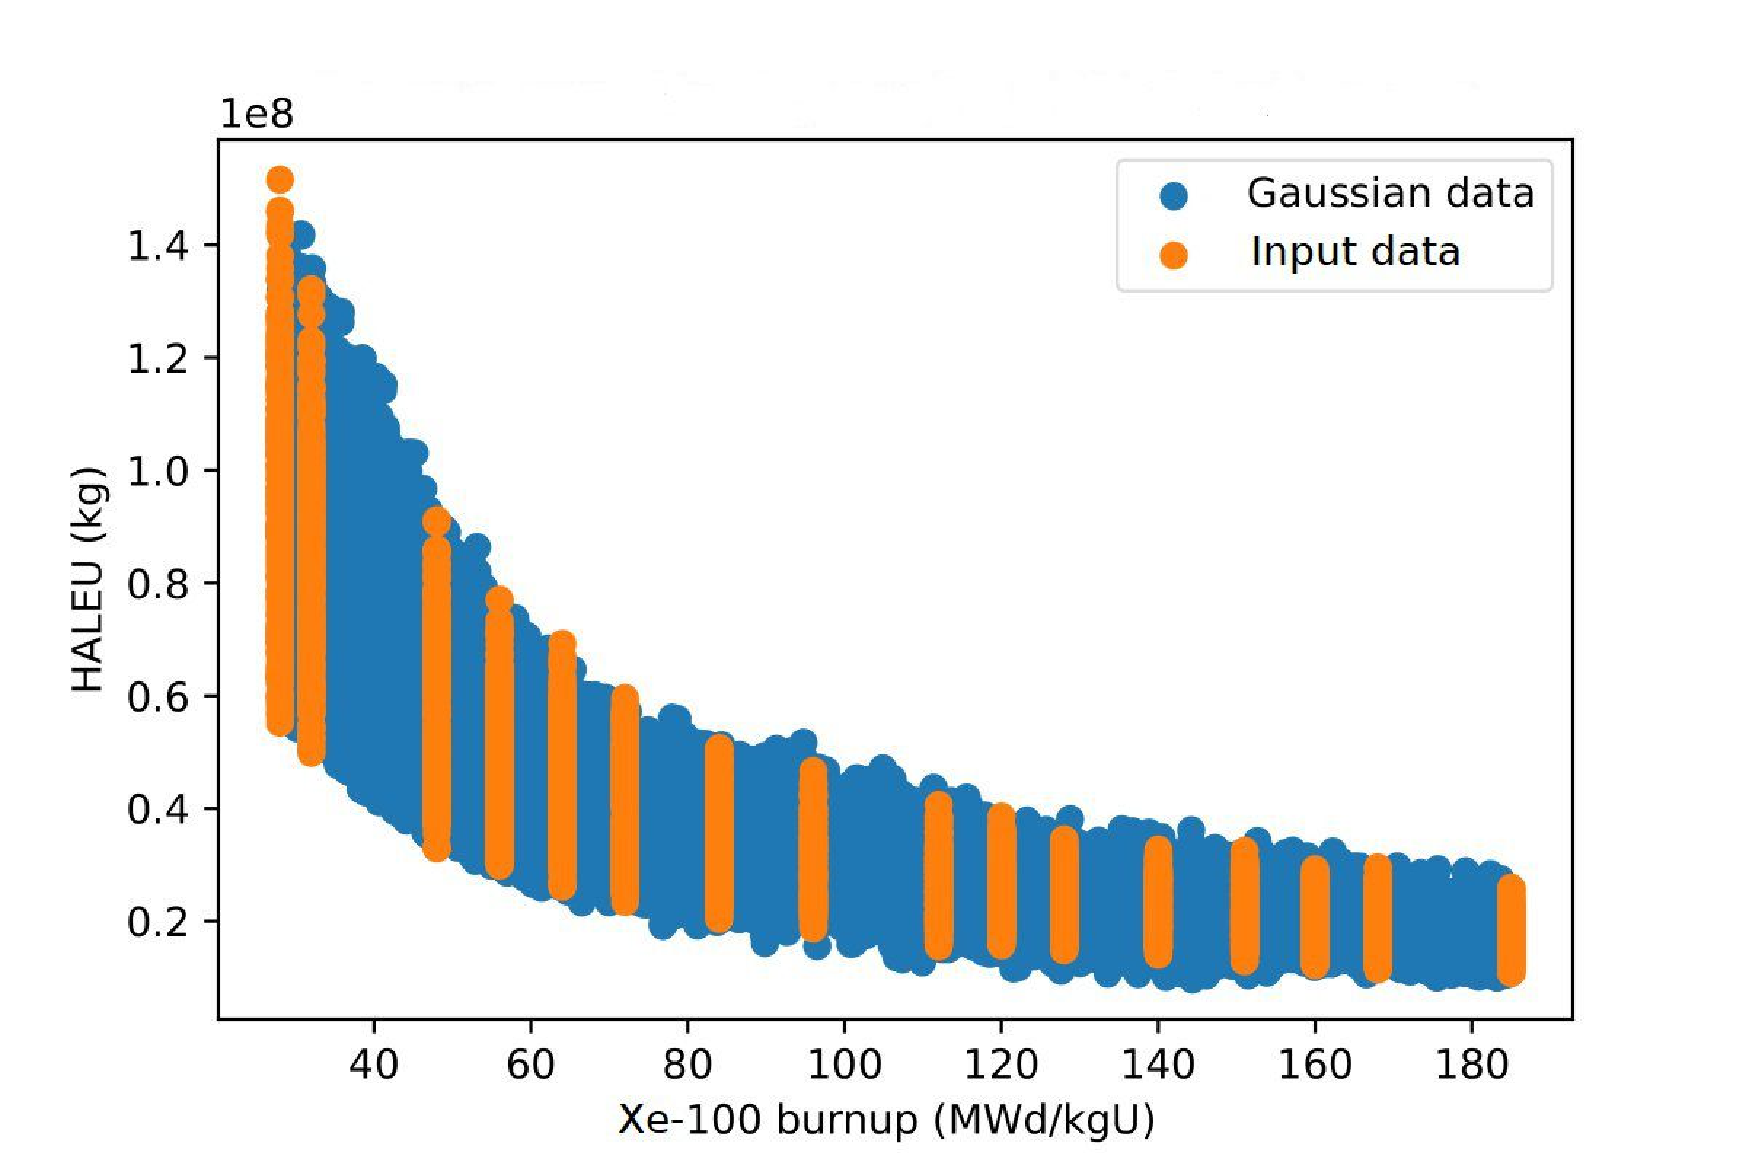
\includegraphics[scale=0.8]{voygr_share_gaussian_xe100_burnup_haleu.pdf}
    \caption{Comparison of the input data and the results of the Gaussian 
    surrogate model when the VOYGR build share is varied.}
    \label{fig:s7_voygr_gaussian}
\end{figure}

The Sobol' indices from this model, shown in Table \ref{tab:s7_sobol_voygr_gaussian}
show a similar trend to the Sobol' indices from varying the \gls{MMR}
build share. The Xe-100 burnup has the largest impact and a large impact 
(a total Sobol' indices greater than 0.5) on all of the 
results. The transition start time and \gls{MMR} burnup have effectively no 
effect on the metrics, and the \gls{LWR} lifetimes and VOYGR build share 
have a very small impact on the metrics. The \gls{LWR} lifetimes has a smaller 
effect on the metrics than when varying the Xe-100 build share, but a similar 
effect on the metrics to when varying the \gls{MMR} build share. 

\begin{table}[h!]
    \centering
    \caption{Sobol' indices for the Gaussian model when varying the VOYGR 
    build share. The first number is the main index, the second is the total 
    index. Highlighted 
    values indicate a total Sobol' indices of above 0.5.}
    \label{tab:s7_sobol_voygr_gaussian}
    \begin{tabular}{c c c c c c c}
        \hline
        & \multicolumn{6}{c}{Output Metric} \\
        Parameter & Fuel Mass & HALEU Mass & SWU & HALEU SWU & Feed & SNF Mass \\
        \hline
        Transition Start & 0.002/0.003 & 0.000/0.001 & 0.000/0.002 & 
                           0.000/0.001 & 0.000/0.001 & 0.001/0.003\\
        LWR Lifetime & 0.065/0.076 & 0.020/0.033 & 0.033/0.045 & 
                       0.020/0.033 & 0.020/0.033 & 0.069/0.081\\
        VOYGR Build Share & 0.252/0.284 & 0.114/0.0151 & 0.028/0.067 &
                            0.114/0.151 & 0.114/0.151 & 0.204/0.238\\
        Xe-100 Burnup & \cellcolor{green!25}0.652/0.683 & \cellcolor{green!25}0.837/0.883 & \cellcolor{green!25}0.910/0.956 & 
        \cellcolor{green!25}0.836/0.881 & \cellcolor{green!25}0.836/0.881 & \cellcolor{green!25}0.696/0.730\\
        MMR Burnup & 0.002/0.002 & 0.000/0.002 & 0.001/0.001 & 
                     0.001/0.002 & 0.001/0.002 & 0.002/0.002\\
        \hline        
    \end{tabular}
\end{table}

Based on the results of the \gls{OAT} analysis, increasing the VOYGR build 
share replaces 
Xe-100s with VOYGRs. Therefore, the VOYGR build share implicitly 
impacts the Xe-100 build share, which leads to this input parameter 
having a larger impact on most of the metrics than most of the other variables. 
The VOYGR build share does not have a noticeable impact on the 
total \gls{SWU} capacity because of the similar \gls{SWU} capacities 
required by the Xe-100 and VOYGR. This result is consistent with the 
Xe-100 build share having a lesser effect on this metric compared 
with its effect on the other metrics. 
The VOYGR build share has a larger impact on the fuel mass and the 
\gls{SNF} mass than the other metrics because the VOYGR takes in more 
and discharges more fuel than the Xe-100 per unit time and energy. 
The 
increased impact of the VOYGR build share on these metrics leads to 
the decreased impact of the Xe-100 burnup, relative to the 
\gls{HALEU}-related metrics. 


\subsubsection{Quadratic surrogate model}
When using the quadratic fit, the R$^2$ values range between 0.94-0.95. 
These values are consistent with the R$^2$ values for the other 
quadratic models in this work. The data from this quadratic model,
compared with the input data in Figure \ref{fig:s7_voygr_quadratic}, 
shows that it does not fully reach the maximum of the input data
and under-predicts some of the minimum values. These trends have 
been observed in all of the quadratic models created for this analysis. 
These trends are a result of the model fitting a second-order 
polynomial to data that does not follow a second order polynomial. This 
mis-fit between the data and the model fit leads to the lower R$^2$ value 
than the Gaussian surrogate models and the inability to properly fit 
to the extremes in the data. Therefore, one would expect the 
Gaussian models to be more accurate in calculating the Sobol' 
indices. The consistency between the values and trends of the 
indices from both models suggests that the quadratic models are 
still sufficient for these purposes. 

\begin{figure}[h!]
    \centering 
    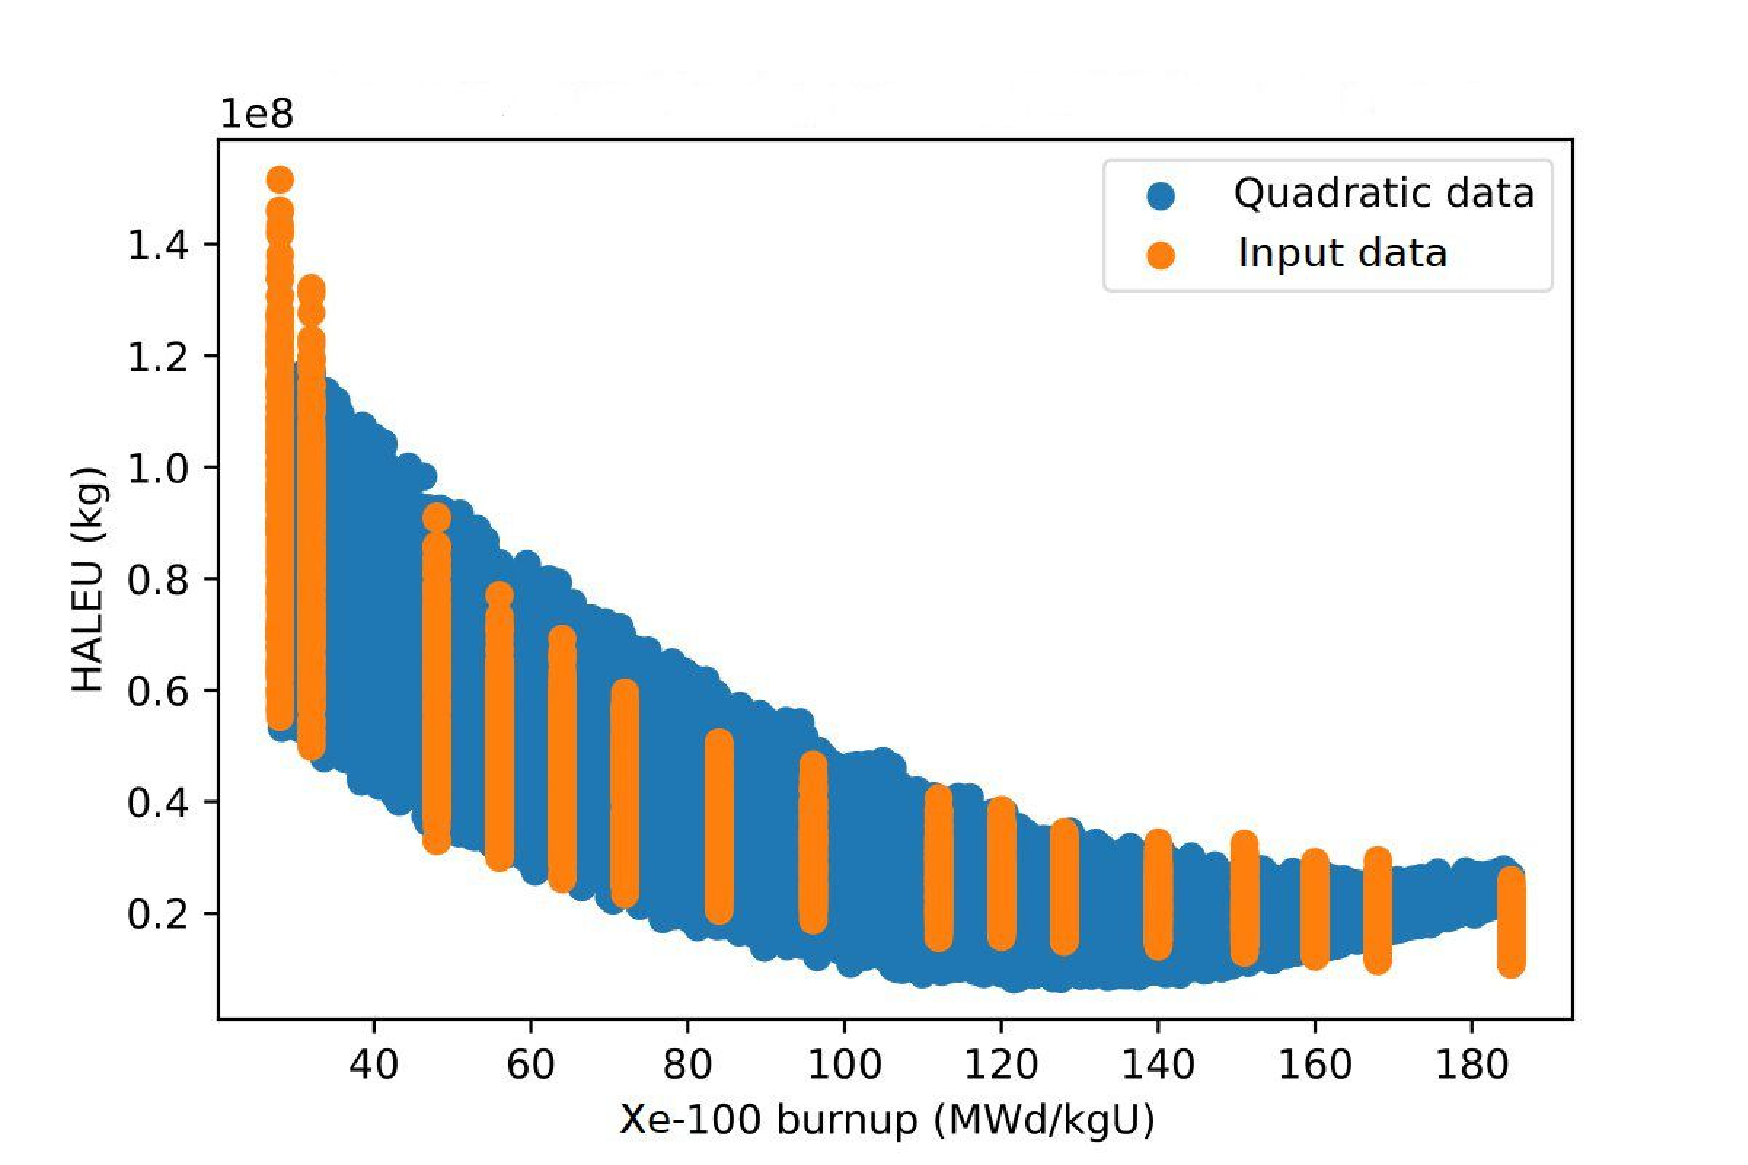
\includegraphics[scale=0.8]{voygr_share_quadratic_xe100_burnup_haleu.pdf}
    \caption{Comparison of the input data and the results of the quadratic 
    surrogate model when the VOYGR build share is varied.}
    \label{fig:s7_voygr_quadratic}
\end{figure}

The Sobol' indices from this model, reported in Table 
\ref{tab:s7_sobol_voygr_quadratic},
have the same pattern as the Sobol' indices from the Gaussian model created. 
The Xe-100 burnup is the most impactful input parameter on all of the 
output metrics, followed by the VOYGR build share and the \gls{LWR} lifetime. 
The transition start time and the \gls{MMR} burnup have a negligible effect 
on the results of the metrics. 

\begin{table}[h!]
    \centering
    \caption{Sobol' indices for the quadratic model when varying the VOYGR 
    build share. The first number is the main index, the second is the total 
    index. Highlighted 
    values indicate a total Sobol' indices of above 0.5.}
    \label{tab:s7_sobol_voygr_quadratic}
    \begin{tabular}{c c c c c c c}
        \hline
        & \multicolumn{6}{c}{Output Metric} \\
        Parameter & Fuel Mass & HALEU Mass & SWU & HALEU SWU & Feed & SNF Mass \\
        \hline
        Transition Start & 0.002/0.002 & 0.000/0.000 & 0.000/0.001 &
                           0.000/0.000 & 0.000/0.000 & 0.001/0.002\\
        LWR Lifetime & 0.063/0.071 & 0.020/0.031 & 0.031/0.042 &
                       0.051/0.031 & 0.020/0.031 & 0.066/0.075\\
        VOYGR Build Share & 0.214/0.243 & 0.108/0.143 & 0.030/0.066 &
                            0.108/0.143 & 0.108/0.143 & 0.170/0.200\\
        Xe-100 Burnup & \cellcolor{green!25}0.700/0.724 & \cellcolor{green!25}0.843/0.884 & \cellcolor{green!25}0.911/0.952 &
        \cellcolor{green!25}0.842/0.883 &\cellcolor{green!25} 0.843/0.883 & \cellcolor{green!25}0.740/0.767\\
        MMR Burnup & 0.001/0.001 & 0.001/0.001 & 0.001/0.002 &
                     0.001/0.002 & 0.001/0.001 & 0.001/0.001\\
        \hline        
    \end{tabular}
\end{table}


